
%\section{How to Use this Template}

%The template details the sections that can be used in a manuscript. Note that the order and names of article sections may differ from the requirements of the journal (e.g., the positioning of the Materials and Methods section). Please check the instructions on the authors' page of the journal to verify the correct order and names. For any questions, please contact the editorial office of the journal or support@mdpi.com. For LaTeX-related questions please contact latex@mdpi.com.
%The order of the section titles is: Introduction, Materials and Methods, Results, Discussion, Conclusions for these journals: aerospace,algorithms,antibodies,antioxidants,atmosphere,axioms,biomedicines,carbon,crystals,designs,diagnostics,environments,fermentation,fluids,forests,fractalfract,informatics,information,inventions,jfmk,jrfm,lubricants,neonatalscreening,neuroglia,particles,pharmaceutics,polymers,processes,technologies,viruses,vision

%%%%%%%%%%%%%%%%%%%%%%%%%%%%%%%%%%%%%%%%%%%%%%%%%%%%%%%%%%%%%%%%%%%%%%%%%%%%%%%%%%%%%%%
\section{Introduction}

%The introduction should briefly place the study in a broad context and highlight why it is important. It should define the purpose of the work and its significance. The current state of the research field should be reviewed carefully and key publications cited. Please highlight controversial and diverging hypotheses when necessary. Finally, briefly mention the main aim of the work and highlight the principal conclusions. As far as possible, please keep the introduction comprehensible to scientists outside your particular field of research.  %Please use the command \citep{} for the following MDPI journals, which use author--date citation: Administrative Sciences, Arts, Econometrics, Economies, Genealogy, Histories, Humanities, IJFS, Journal of Intelligence, Journalism and Media, JRFM, Languages, Laws, Religions, Risks, Social Sciences.


Supercritical CO$_2$ Brayton cycles are promising cycle configurations offering higher efficiencies, compact design, and reduced turbomachinery cost while operating with non toxic working fluid. Various sCO$_2$ Brayton cycles have been modeled with the recompression cycle having efficiency advantages over other proposed cycle arrangements \cite{turchi_2013,ahn_2014,wang_2018}. The literature shows that the recompression cycle can reach efficiencies of 50\% in some scenarios (with turbine inlet temperatures in the 650-700 $^{\circ}$C range) \cite{turchi_2013,wright_2009}, allows these cycles to be a competitive alternative to steam Rankine and air Brayton cycles over a range of temperatures.   Due to the benefits of sCO$_2$ Brayton cycles, the United States Department of Energy is investigating these conversion cycles for use with heat sources including nuclear and solar \cite{doe_2012}. Multiple project funding opportunities are established with the National Energy Technology Laboratory offering 144 million dollar award for demonstration and performance verification of a sCO$_2$ Brayton cycle \cite{netl_2016} and the Office of Energy Efficiency \& Renewable Energy offering 2.6 million dollar reward in their Brayton Energy project for a integrated CSP receiver, TES, and power block in one sCO$_2$ Brayton system \cite{seto_2015}. Utilizing complementary technologies, specifically solar concentrating power and lead-cooled fast reactors, can offset the drawbacks of each. Coupling these technologies into an interconnected cycle allows for consistent generation, independent of weather or time of day, and thermal storage for high dispatchability during high grid demand periods.
A CSP has an array of mirrors concentrating solar rays towards a receiver to generate thermal energy therefore causing a dependency on weather conditions and time of day. Previous research has modeled CSP technology as the thermal source for Brayton sCO$_2$ cycles with promising results in efficiency gains and high temperature thermal energy storage \cite{turchi_2013, iverson_2013, ho_2015, wang_2018, neises_2020}. Thermal energy gathered from the CSP is stored in thermal energy storage which is dispatched into the sCO$_2$ Brayton cycle when grid demand increases. With a comparable temperature to the hot TES, 560 $^{\circ}$C, a LFR is capable of transferring heat to thermal storage for later dispatch. An LFR uses fission reactions to heat a heat transfer fluid, in this case liquid lead, to temperatures of 650 $^{\circ}$C. Nuclear sCO$_2$ Brayton cycles have been studied with similar gains in efficiency seen in CSP sCO$_2$ Brayton cycles \cite{ dostal_2004, luo_2020}. Physical testing of simple sCO$_2$ Brayton cycles has been performed at Sandia National Laboratories \cite{wright_2011} and in Korea \cite{cha_2016}, with at least two commercial companies (Echogen, Net Power) having progressed to building pilot cycles  \cite{held_2015,fetvedt_2016}. 

Various studies on complimentary solar-nuclear systems have been accomplished with several reviewed as follows: 

\begin{itemize}
    \item	Monnerie et al. (2011): In search of an alternative to the typical fossil fuel-based process, reports on synthesizing hydrogen with complimentary solar-nuclear technologies being utilized as consistent heat sources for chemical decomposition of sulphuric acid to aid in simple, low-temperature electrolysis \cite{monnerie_2011}. 
    \item   Curtis J.D. (2015): Massachusetts Institute of Technology thesis reports cycle configuration, performance, and development of complimentary solar-nuclear systems with a focus on shale oil extraction and production from kerogen deposits \cite{curtis_2015}. 
    \item   Wang et al. (2020): Implements a combined solar and nuclear plant discussing a sCO$_2$ Brayton recompression cycle layout with an emphasis on a cycle design's performance to varying solar irradiance and demonstration of feasibility \cite{wang_2020}. 
\end{itemize}

The economic and physical feasibility of producing shale oil and hydrogen with complimentary solar-nuclear cycles, as discussed in the Curtis J.D. (2015) thesis and Monnerie et al. (2011) article, is not within the scope of sCO$_2$ Brayton recompression cycle electrical generation and storage presented in this paper.

The single cycle configuration in Wang et al. (2020) has a higher-temperature operating salt, 67\%KCl-33\%MgCl$_2$, as the heat transfer fluid in the CSP which is capable of temperatures in the range of 450 - 1400 $^{\circ}$C. The lower operating point of the studied solar salt in this paper, 60\%NaNO$_3$-40\%KNO$_3$ with a temperature range of 250 - 585 $^{\circ}$C, is employed because the technology is more established when compared to KCl-MgCl$_2$ \cite{turchi_2018}. The higher temperature salt requires preheating which is achieved prior to the CSP heat addition by a small modular lead-cooled fast reactor. The small modular LFR operates at a low temperature and a fixed location when compared to the higher temperature lead and variable location that the Westinghouse LFR studied in this paper is capable of. Due to the similar operating temperatures of the CSP and LFR, multiple cycle configurations are studied that are not possible with the similar components in Wang et al. (2020). Specifically studied in this paper are the effects on cycle and heat storage efficiency of different cycle configurations while having the LFR serve a dual purpose of electrical generation and a supplementary CSP TES charging technique. This paper provides an overview of contending recompression sCO$_2$ Brayton cycles with varied positioning of complimentary CSP and LFR heat additions in the cycle. Additionally the location of where heat is drawn from the sCO$_2$ Brayton cycles to be stored in thermal energy storage is studied with the results discussed.



 
%%%%%%%%%%%%%%%%%%%%%%%%%%%%%%%%%%%%%%%%%%%%%%%%%%%%%%%%%%%%%%%%%%%%%%%%%%%%%%%%%%%%%%%
\section{Materials and Methods}

%Materials and Methods should be described with sufficient details to allow others to replicate and build on published results. Please note that publication of your manuscript implicates that you must make all materials, data, computer code, and protocols associated with the publication available to readers. Please disclose at the submission stage any restrictions on the availability of materials or information. New methods and protocols should be described in detail while well-established methods can be briefly described and appropriately cited.

%Research manuscripts reporting large datasets that are deposited in a publicly avail-able database should specify where the data have been deposited and provide the relevant accession numbers. If the accession numbers have not yet been obtained at the time of submission, please state that they will be provided during review. They must be provided prior to publication.

%Interventionary studies involving animals or humans, and other studies require ethical approval must list the authority that provided approval and the corresponding ethical approval code.
%\begin{quote}
%This is an example of a quote.
%\end{quote}

% **************************************


\subsection{Cycle Component Modeling}
%======================================================================================
Components present in the cycles are modeled using various techniques and are discussed in more detail below. Turbines and compressors are analyzed using isentropic efficiencies. Counter-flow heat exchangers are modeled using the effectiveness-NTU method while simplified ``black box'' heat exchangers that use a simple energy balance for state point calculations are used in lieu of more detailed component models where data is available. The lead-cooled fast reactor is assumed to be a black box heat exchanger because of the constant heat input and state points on the sCO$_2$ inlet and outlet are provided. The molten salt loop for the CSP is modeled with necessary components including hot and cold TES, receiver, pumps and counter-flow heat exchangers.



\subsubsection{Turbines and Compressors }
%--------------------------------------------------------------------------------------

Turbines and compressors are modeled for each cycle using constant isentropic efficiency values which are summarized in Table \ref{tab-cycle-constants}. Turbines take the high pressure sCO$_2$ and expand it through a series of blades allowing a production of energy, while compressors input mechanical energy to increase the pressure of the sCO$_2$. The turbines and compressors are assumed to be at steady state, exchange no heat with the surroundings, and have single inlet and outlet streams. Using this estimate, along with a known low and high side pressures, temperature and enthalpy outlets of the turbine and compressor are calculated \cite{klein_nellis_2011}. 

\subsubsection{Black Box and Counter-Flow Heat Exchangers}
%--------------------------------------------------------------------------------------

Black box heat exchangers are simplified heat exchangers which have no approach temperature or pinch point and are modeled as a perfect heat transfer into or out of the cycle. These heat exchangers use an energy balance with mass flow inlet energy, heat input or output, and mass flow outlet energy. The energy balance equation used for all black box heat exchangers is Equation \ref{eq-black}.


\begin{equation}
    \label{eq-black}
    \dot{m} \cdot h_{in} + \dot{Q}_{HX} = \dot{m} \cdot h_{out} ,
\end{equation}

In this equation the energy input to the system is on the left hand side with $\dot{m}$ multiplied by $h_{in}$ being energy from the mass flow while $\dot{Q}_{HX}$ is heat transfer directly into, positive, or out of, negative, the flow from an outside source. The right hand side of the equation is heat leaving the black box heat exchanger with $\dot{m}$ and enthalpy of $h_{out}$. Black box energy balances are used in three situations, the receiver, LFR heat exchanger, and pre-cooler heat exchanger. These heat exchangers are not exhaustively modeled because the state points on the inlet and outlet are defined by design parameters.

Counter-flow heat exchangers are modeled with two fluids flowing in opposite directions exchanging heat from the hot side to the cold side. The temperatures of the hot and cold flows on either side of the the heat exchanger have a temperature difference known as an approach temperature. A diagram showing a simplified counter-flow heat exchanger is illustrated in Figure \ref{counter-flow-hx}.

% \end{paracol}
\begin{figure}[h]
    \widefigure
    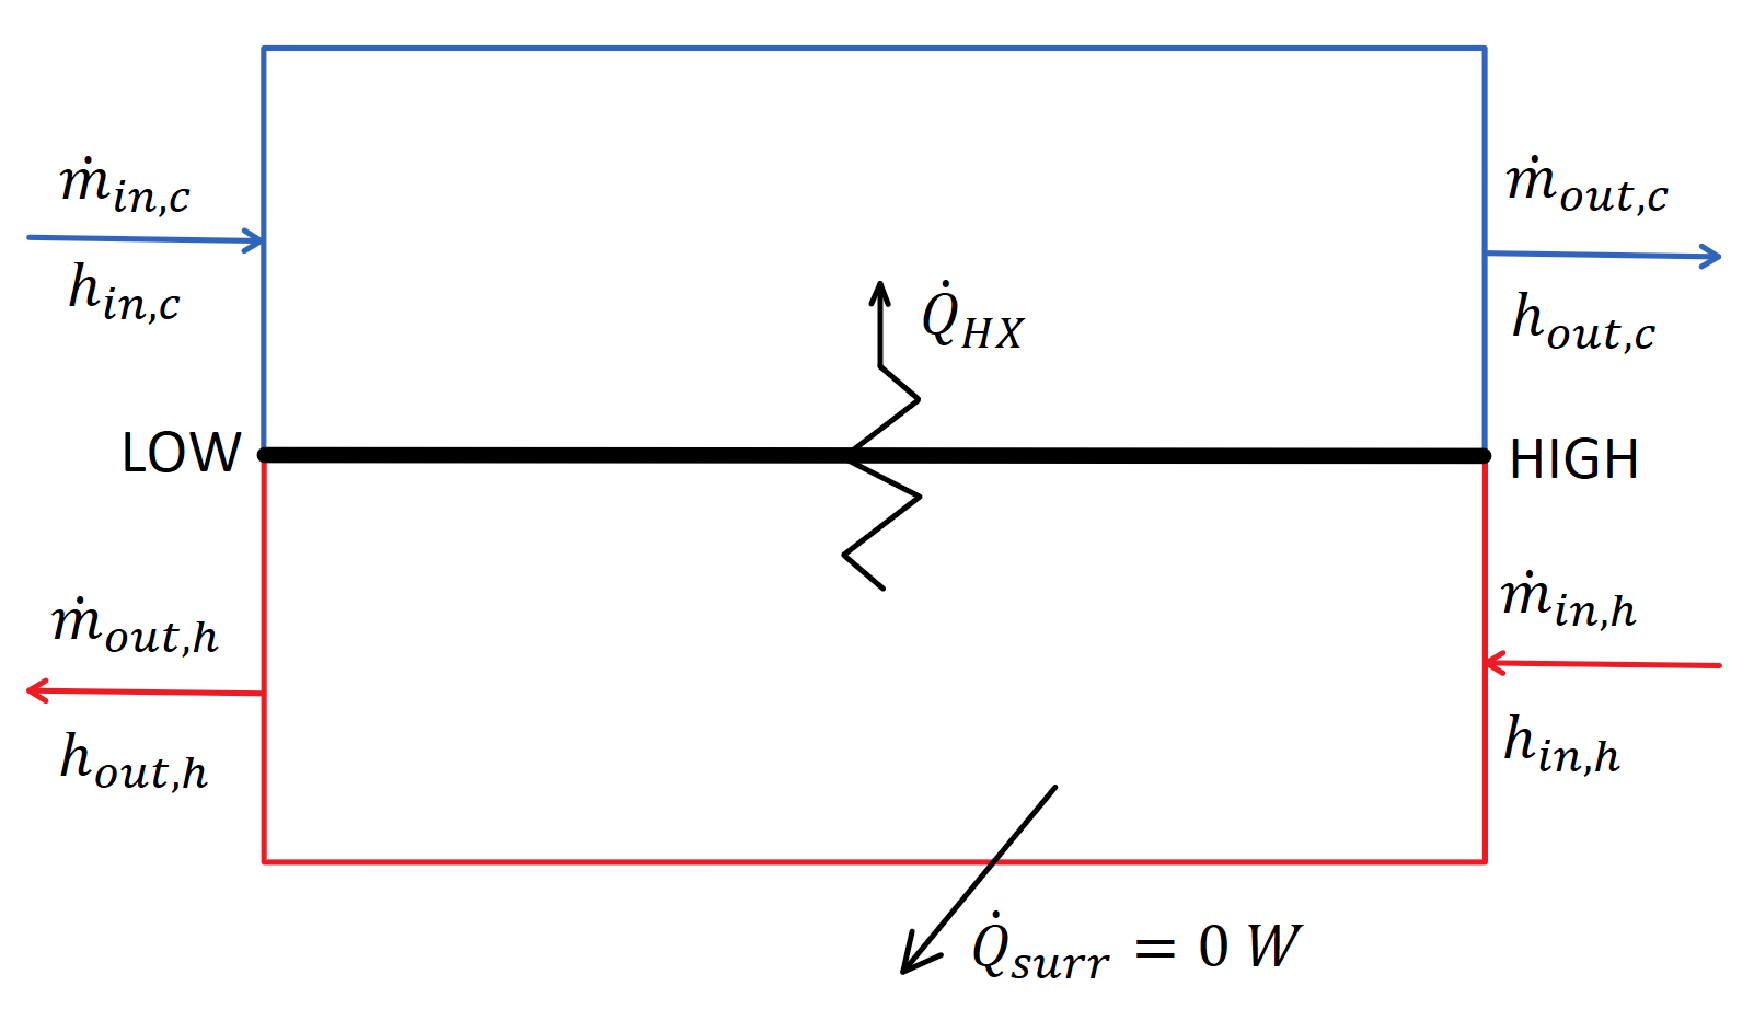
\includegraphics[width=10 cm]{Definitions/counter-flow-hx.pdf}
    \caption{Simplified counter-flow heat exchanger diagram. \label{counter-flow-hx}}
\end{figure}
% \begin{paracol}{2}
% \linenumbers
% \switchcolumn

Additional assumptions of the counter-flow heat exchanger model are: no heat loss to the surroundings, no pressure drops across the heat exchangers, and no fouling resistances. In Figure \ref{counter-flow-hx} the subscript 'out' denotes where the streams are leaving, 'in' denotes the entering streams, 'c' and 'h' signify cold and hot streams respectively, $\dot{Q}_{HX}$ is the total heat transfer from the hot to cold stream, and $\dot{Q}_{surr}$ is the heat transfer to the surroundings.

Counter-flow heat exchanger calculations require two known state points, fluid properties, mass flow rate of hot and cold side, and a specified approach temperature. In the modeled cases, the approach temperature is set to value of $10^{\circ}$C, based off prior model development of sCO$_{2}$ Brayton cycle heat exchangers \cite{seidel_2010_model_development}. The fluid libraries referenced are built into EES for Carbon Dioxide and Salt (60\% NaNO$_3$ 40\% KNO$_3$) \cite{pacheco_1995_salt_properties,roland_1996_co2_properties}. 

To analyze the counter-flow heat exchanger a side is chosen, usually the high side, to start the calculations. The approach temperature is initially subtracted from the hot stream on the high temperature side to find the missing cold temperature according to Equation \ref{temp_h}. 

\begin{equation}
   \label{temp_h}
    T_{out,c} = T_{in,h}-\Delta_{T},
\end{equation}

Where T$_{out,c}$ is the cold stream outlet temperature and T$_{in,h}$ is the hot stream inlet temperature. Knowing the two state points allows for the enthalpy out to be found using correlations from the fluid property libraries. This enthalpy then allows for the heat transfer of the heat exchanger to be found with Equation \ref{heattrans_h}.

\begin{equation}
    \label{heattrans_h}
     \dot{Q}_{HX} = \dot{m}_{c}(h_{out,c}-h_{in,c}),
 \end{equation}

 Where $\dot{Q}_{HX}$ is the total heat transfer rate from the hot stream to the cold stream, $\dot{m}_{c}$ is the mass flow rate of the cold stream, $h_{out,c}$ is the enthalpy at the outlet of the cold side, and $h_{in,c}$ is the inlet of the cold side.
 The known heat transfer of the counter-flow heat exchanger can then solve for the enthalpy out of the hot stream, h$_{out,h}$. This is accomplished with Equation \ref{enthalpy_h}.

 \begin{equation}
    \label{enthalpy_h}
     h_{out,h} = h_{in,h} - \frac{\dot{Q}_{HX}}{\dot{m}_{h}},
 \end{equation}

Knowing the hot stream enthalpy out allows for all states to be set on the outlets and inlets of the counter-flow heat exchanger. The temperature difference of the low side is then checked to ensure that it is larger than the approach temperature, defined at $10^\circ$C. If the temperature difference on the low side is smaller than the approach temperature, the same computations are carried with the low side as the starting point.

Knowing the state points on all inlets and outlets of the counter-flow heat exchanger allows for the heat exchanger performance metrics to be calculated. Performance metrics include effectiveness, capacitance ratio, UA, and NTU for heat exchangers. Effectiveness is the ratio of the actual heat transfer rate to the maximum heat transfer rate, or a perfect heat exchanger with no approach temperature. Assuming the approach temperature is on the high side, the maximum heat transfer rate, $\dot{Q}_{max}$ is found with the maximum enthalpy. Maximum enthalpy of the cold stream is found with correlations by setting the temperature to T$_{in,h}$ with same pressure on the cold outlet. Using the maximum enthalpy, $h_{max}$, the maximum heat transfer rate is calculated using Equation \ref{heattrans_max}.

\begin{equation}
    \label{heattrans_max}
    \dot{Q}_{max} = \dot{m}_{c}(h_{max}-h_{in,c}),
\end{equation}

Calculating the maximum heat transfer rate allows for effectiveness to be calculated using the ratio in Equation \ref{effective}.

\begin{equation}
    \label{effective}
    \varepsilon = \frac{\dot{Q}_{HX}}{\dot{Q}_{max}},
\end{equation}

All of the prior equations are carried out in a built-in function within EES. EES is an iterative solver, therefore as long as there is a feasible solution, the functions can take any of the four state points around the heat exchanger and converge on a solution.

After the effectiveness is solved for, capacitance ratio is necessary. The capacitance ratio is defined as the average minimum capacitance rate, $\dot{C}_{min}$, over the average maximum capacitance rate, $\dot{C}_{max}$. Average capacitance rates for the hot and cold streams are found by multiplying the addition of the specific heat at the inlet and outlet of the stream by the mass flow and dividing by two as seen in Equation \ref{avg_cap}.

\begin{equation}
    \label{avg_cap}
    \dot{C}_{avg} = \frac{\dot{m}(c_{in}+c_{out})}{2},
\end{equation}

Where $C_{avg}$ is the average capacitance rate across the hot or cold stream and $c_{in}$ and $c_{out}$ is the specific heat at the inlet and outlet respectively. Specific heat is found using library correlations. Once both average capacitances are calculated for the hot and cold streams, one has a larger value, $\dot{C}_{max}$, and one has a smaller value,  $\dot{C}_{min}$. These maximum and minimum values are used to find the capacitance ratio, $CR$, in Equation \ref{cap_ratio}.

\begin{equation}
    \label{cap_ratio}
    CR = \frac{\dot{C}_{min}}{\dot{C}_{max}},
\end{equation}


\subsubsection{Lead-Cooled Fast Reactor}
%--------------------------------------------------------------------------------------
Lead-cooled fast reactors use energy from a controlled nuclear reaction to heat molten lead. This lead is used to cool the core and transfer heat into the sCO$_2$ Brayton power cycle \cite{smith_2016_lfr_background,alemberti_2013_lfr_overview}. The lead-cooled fast reactor is assumed to be a black box heat transfer and is labeled in the cycle models LFR HX. The inlet, outlet and heat transfer rates are provided by our industry partner, Westinghouse, making the black box simplification viable. The energy balance for the black box assumption can be seen in Equation \ref{eq-lfr-black-box}.

\begin{equation}
    \label{eq-lfr-black-box}
    \dot{m} \cdot h_{inlet} + \dot{Q}_{LFRHX} = \dot{m} \cdot h_{outlet},
\end{equation}

Where the left hand side, $\dot{m}$, $h_{inlet}$, and $\dot{Q}_{LFRHX}$, is the energy into the flow and the right hand side, $\dot{m}$ and $h_{outlet}$, is the energy brought out from the flow of sCO$_2$. The amount of energy transferred into the cycle, $\dot{Q}_{LFRHX}$, is set at $950$ MW, and outlet temperature of the sCO$_2$ from the LFR HX is set at a value of $595^{\circ}$C. The outlet temperature of the LFR is specified because of high temperature material limits on the LFR lead side. The low temperature side is allowed to vary over a range of values with some considerations. The lead flow velocity is limited by the erosion of the fuel, the slower the lead flow velocity reduces fuel erosion and therefore leads to a more desirable compact design. Restricting the lead flow velocity, and therefore lead mass flow rate, leads to a higher LFR power output when the inlet sCO$_2$ temperature is reduced. LFR sCO$_2$ inlet temperature has a lower bound of $340^{\circ}$C before the lead begins to freeze, which is operationally unacceptable. When the inlet temperature of sCO$_2$ is increased the temperature difference across the LFR is decreased leading to an increase in power conversion cycle thermodynamic efficiency but a reduction in LFR power below $950$ MW. There is a compromise between high LFR efficiency and LFR power, therefore a temperature of $400^{\circ}$C for the sCO$_2$ inlet temperature is the optimal value provided by Westinghouse.


\subsubsection{Concentrating Solar Power Cycle}
%--------------------------------------------------------------------------------------

The CSP salt cycle modeled in this paper is composed of hot and cold thermal energy storage (TES), pumps, receiver, sCO$_2$-to-salt counter-flow heat exchanger (C2S), and CSP counter-flow heat exchanger (CSP HX). The diagram for this CSP salt loop is seen in Figure \ref{csp}. 

% \end{paracol}


\begin{figure}[h] 
    %[htb]
    \widefigure
    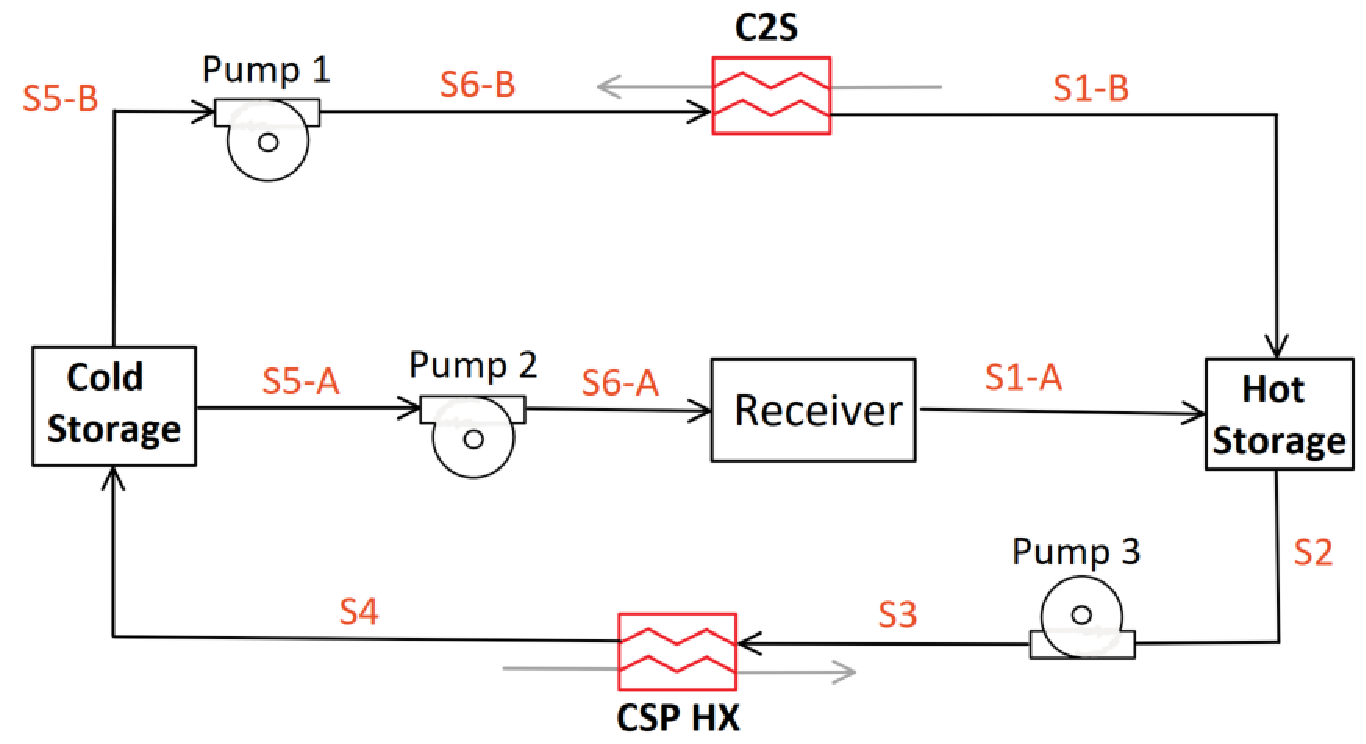
\includegraphics[width=10 cm]{Definitions/csp.pdf}
    \caption{Diagram for CSP cycle with cold and hot thermal energy storage, pumps, and csp black box heat input\label{csp}}
\end{figure}
% \begin{paracol}{2}
% \linenumbers
% \switchcolumn

The CSP salt cycle uses 60\% sodium nitrate, NaNO$_3$, and 40\% potassium nitrate, KNO$_3$, 'solar salt' as the heat transfer fluid. Solar salt stored in the hot TES can be dispatched on demand through the CSP HX when grid demand increases and held when grid demand is low. Current CSP salt cycles heat solar salt with receivers and store it in hot TES tanks at temperatures around 565$^{\circ}$C. Future CSP salt cycles are hypothesized to have bulk hot TES temperatures of up to $720^{\circ}$C, but here the hot TES temperature is set at $560^{\circ}$C for all modeled cycles \cite{mehos2017concentrating} as this has been commercially proven. The cold TES temperature takes on three different values according to cycle configuration capabilities: $390^{\circ}$C, $410^{\circ}$C, and $440^{\circ}$C. In addition to the lower hot TES temperature, current CSP salt cycles lack a secondary option for charging the hot TES \cite{hamilton2020dispatch}. The studied CSP salt cycle has two TES charging options: a receiver, which generates heat from a heliostat field, and C2S heat exchanger, which draws excess heat from the sCO$_2$ Brayton cycle. While the hot TES is charging, the receiver and LFR are storing heat for later use when grid demand increases. The hot TES storage is not dispensing salt for use in the CSP cycle while charging.

The C2S heat exchanger is active in the 'charging' cycle operating modes, when the focus is on heat storage for later use. Pump 1 is actively moving solar salt from cold TES to hot TES through the C2S heat exchanger extracting heat from the sCO$_2$ Brayton cycle. Additionally, while the focus is on heat storage, and the heliostat field is inputting heat, pump 2 is actively transporting solar salt through the receiver to be stored in the hot TES.

'Non-charging' cycle operating modes are characterized by operations wherein the CSP salt cycle is discharging the hot TES, the C2S heat exchanger is not transferring heat, and the LFR is dispatching heat directly to generate electricity. When electrical generation is occurring and solar resource is available, the heat input in the CSP salt cycle is modelled through a black box energy balance across states S6-A and S1-A with a heat addition of 750 MW from the heliostat field. The hot TES solar salt is moved through Pump 3 and transfers heat into the sCO$_{2}$ Brayton cycle through CSP HX to be converted into electricity. The cooled salt is stored in cold storage and moved through Pump 2 where the heat from the receiver is again transferred into the CSP cycle. 

When grid demand for electrical power increases, a series of operating modes are activated. During the highest demand times, cycle operation focuses on maximum electrical generation. This is achieved through the C2S being turned off for direct electrical production from the LFR and the hot TES is discharging heat through the CSP HX for electrical production in the sCO$_2$ Brayton cycle. As grid demand diminishes, CSP HX ramps down heat extraction until no power is being dispatched through the salt and the hot TES begins charging. During this process, the LFR gradually adds a larger fraction of heat input to the TES through C2S. This process continues until no electrical production is occurring in the cycle and all heat is stored in TES for later use.



\subsection{Standardization of Cycle Modeling}
%======================================================================================


In order to draw a more direct comparison, the cycles are standardized in terms of isentropic efficiencies, heat exchanger approach temperatures, pressures, heat input, and pump constants. These values are summarized in Table \ref{tab-cycle-constants}.

\begin{specialtable}[H] 
    %[htbp]
    \caption{Standardized constant cycle parameters with definition, variable and set value. \label{tab-cycle-constants}}
    \begin{tabular}{L{0.5\linewidth}cc}
    \toprule
    \textbf{Parameter} & \textbf{Variable}	& \textbf{Design Point Value}\\
    \midrule
    \textit{Efficiencies}\\
    Main Compressor & $\eta_{MC}$		& 0.91 (-)\\
    Re-Compressor & $\eta_{RC}$		& 0.89 (-)\\
    Turbine & $\eta_{T}$		& 0.90 (-)\\
    Pumps 1-3 & $\eta_{P}$      & 0.90 (-)\\
    \midrule
    \textit{Approach Temperatures}\\
    Low Temperature Recuperator & $\delta_{LTR}$		& 10 ($^{\circ}$C)\\
    High Temperature Recuperator & $\delta_{HTR}$		& 10 ($^{\circ}$C)\\
    Concentrating Solar Power Heat Exchanger & $\delta_{CSPHX}$	& 10 ($^{\circ}$C)\\
    \midrule
    \textit{Pressures}\\
    Pressure Ratio & $PR$ & 3.27 (-)\\
    High Side Pressure & $P_{2A}$ & 28.8 (MPa)\\
    \midrule
    \textit{Heat Into System}\\
    Lead-Cooled Fast Reactor Heat Transfer & $\dot{Q}_{LFRHX}$ & 950 (MW)\\
    Concentrating Solar Power Heat Transfer & $\dot{Q}_{CSP}$ & 750 (MW)\\
    \midrule
    \textit{Temperature}\\
    Main Compressor Inlet & $T_{1A}$ & 40 ($^{\circ}$C)\\
    Lead-Cooled Fast Reactor sCO$_{2}$ High Temperature & $T_{5}$,$T_{2C}$,$T_{6A}$,$T_{5C}$ & 595 ($^{\circ}$C)\\
    \midrule
    \textit{Pumps}\\
    Pressure Rise Across Pump & $\Delta_{P}$ & 3.726 (MPa)\\
    Pump Low Side Pressure & $P_{S5-B}$ & 3 (MPa)\\ 
    \bottomrule
    \end{tabular}
\end{specialtable}

The values displayed in Table \ref{tab-cycle-constants} are representative of CSP and the Westinghouse LFR.


In addition to standardized parameters, all cycles have identical recompression sides. The recompression side contains a precooler, low temperature recuperator, and two compressors; main compressor and recompressor. 
The modeled cycles are summarized in Table \ref{tab-cycle_sum}.

\begin{specialtable}[H] 
    \caption{Summary of all modeled non-charging and charging cycles with descriptions. \label{tab-cycle_sum}}
    \begin{tabular}{lL{0.7\linewidth}}
    \toprule
    \textbf{Cycle Label} & \textbf{Description}\\
    \midrule
    \textit{Non-Charging}\\
    C-LFR-ON & Two-cycle configuration with LFR as heat source.\\
    C-CSP-ON & Two-cycle configuration with CSP as heat source.\\
    C-1HTR1T-ON & CSP and LFR heat sources in parallel with one turbine.\\
    C-2HTR3T-ON & CSP and LFR loops each with dedicated HTR and turbine.\\
    \midrule
    \textit{Charging}\\
    C-LFR-PRE & Turbine is prior to the C2S.\\
    C-LFR-POST & Turbine is after the C2S.\\
    C-LFR-PAR & Turbine is parallel to the C2S.\\
    C-LFR-CIRC & Circulator bridges the LFR and C2S.\\
    \bottomrule
    \end{tabular}
\end{specialtable}

\subsection{Non-Charging Cycle Configurations} 
%======================================================================================

Various cycles are modeled to test their advantages and disadvantages. These cycle models fall into two categories: non-charging and charging. The non-charging category is used to determine the configuration of the cycle with a focus on electricity generation. This includes the number and location of turbines, recuperators, and heat input to the system by the CSP and LFR. To quantify the effectiveness of the non-charging configurations, a cycle efficiency, $\eta_{cycle}$, is defined in Equation \ref{eq-eta-cycle}.

\begin{equation}
    \label{eq-eta-cycle}
    \eta_{cycle} = \frac{\dot{W}_{T}-\dot{W}_{MC}-\dot{W}_{RC}}{\dot{Q}_{LFRHX}+\dot{Q}_{CSPHX}},
\end{equation}

The numerator in Equation \ref{eq-eta-cycle} is the alternator power, or the power produced from the turbines, $\dot{W}_{T}$, minus the required power of the compressors, $\dot{W}_{MC}$ and $\dot{W}_{RC}$. The denominator is the total power input into the system from the LFR HX, $\dot{Q}_{LFRHX}$, and CSP HX, $\dot{Q}_{CSPHX}$.


\subsubsection{Two-Cycle Configuration: C-LFR-ON and C-CSP-ON} %--------------------------------------------------------------------------------------

The two-cycle configuration that is tested has independent sCO$_{2}$ loops that share a common CSP salt cycle. This cycle has two sCO$_{2}$ Brayton Cycles: C-LFR-ON and C-CSP-ON. Configuration of components for these two cycles is identical with the exception of heat inputs. C-LFR-ON has heat provided from a LFR while C-CSP-ON has heat provided from the CSP. These two cycles individually operate when the focus of plant operation is primarily electricity generation. 
    
The cycle that is using the LFR heat input in the two-cycle configuration is labeled as C-LFR-ON and the cycle diagram is illustrated in Figure \ref{c-lfr-on}. 

% \end{paracol}
\begin{figure}[H] 
    %[!h] 
    \widefigure
    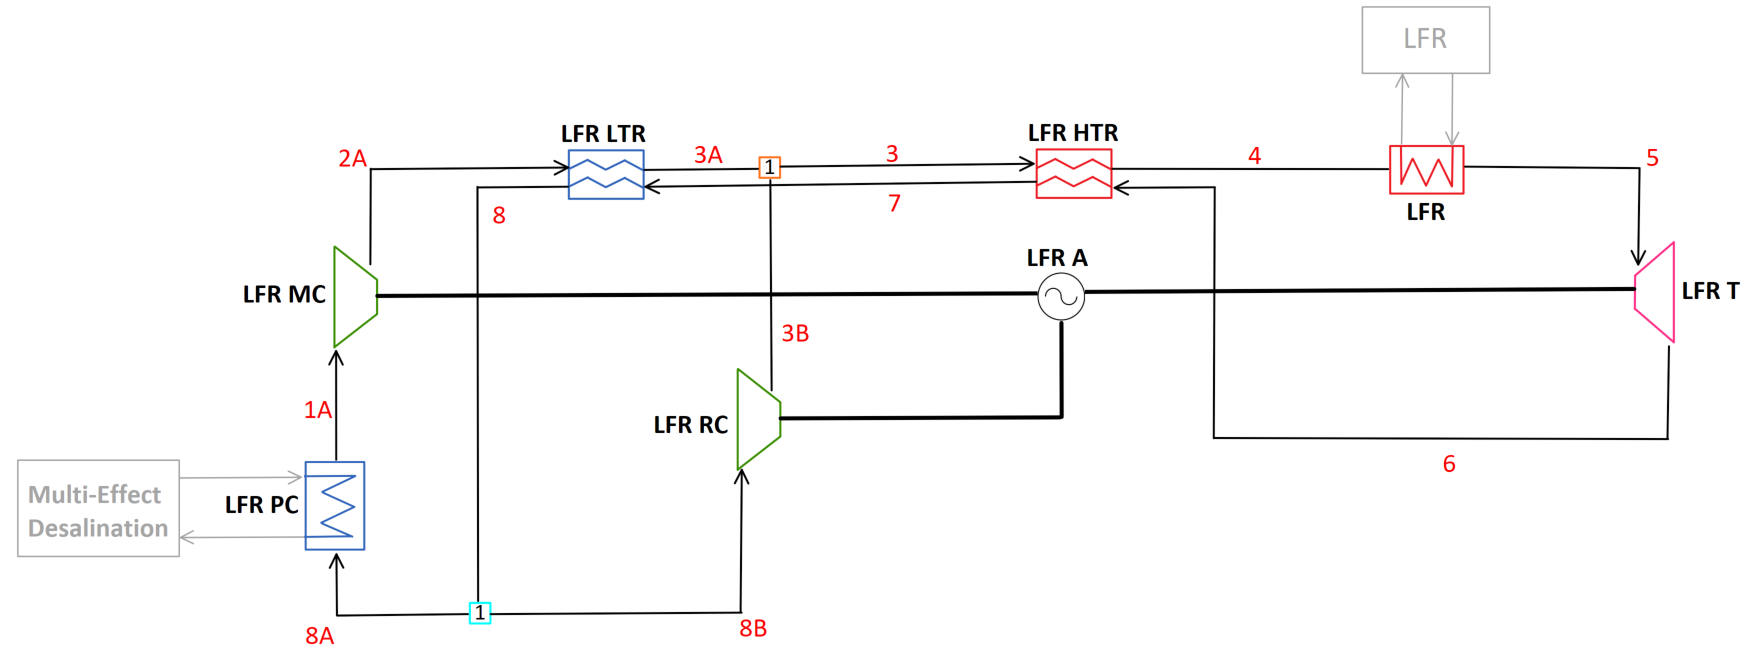
\includegraphics[width=\linewidth]{Definitions/c-lfr-on.pdf}
    \caption{Diagram for C-LFR-ON with focus on electricity generation\label{c-lfr-on}}
\end{figure}
% \begin{paracol}{2}
% \linenumbers
% \switchcolumn

Two separate sensitivity studies on the LFR inlet temperature are completed for C-LFR-ON. The constrained study is calculated by setting the LFR inlet temperature to the design value of $400^{\circ}$C, which is a requirement of the LFR primary circuit to maximize power output within material limits. In addition to the constrained studies, unconstrained studies are required to test the penalties that LFR inlet temperature has on efficiency. The unconstrained study is performed by gradually increasing the mass flow to the main compressor through a parametric study while maximizing cycle efficiency. In Figure \ref{c-lfr-on}, the location of the C2S heat exchanger while charging falls between state point 5 and 6 in any of the studied charging configurations: parallel, pre, circulator or post. 

The cycle that is using the CSP heat input in the two-cycle configuration is labeled C-CSP-ON and the cycle diagram is shown in Figure \ref{c-csp-on}. 

\end{paracol}
\begin{figure}[H] 
    %[!h]
    \widefigure
    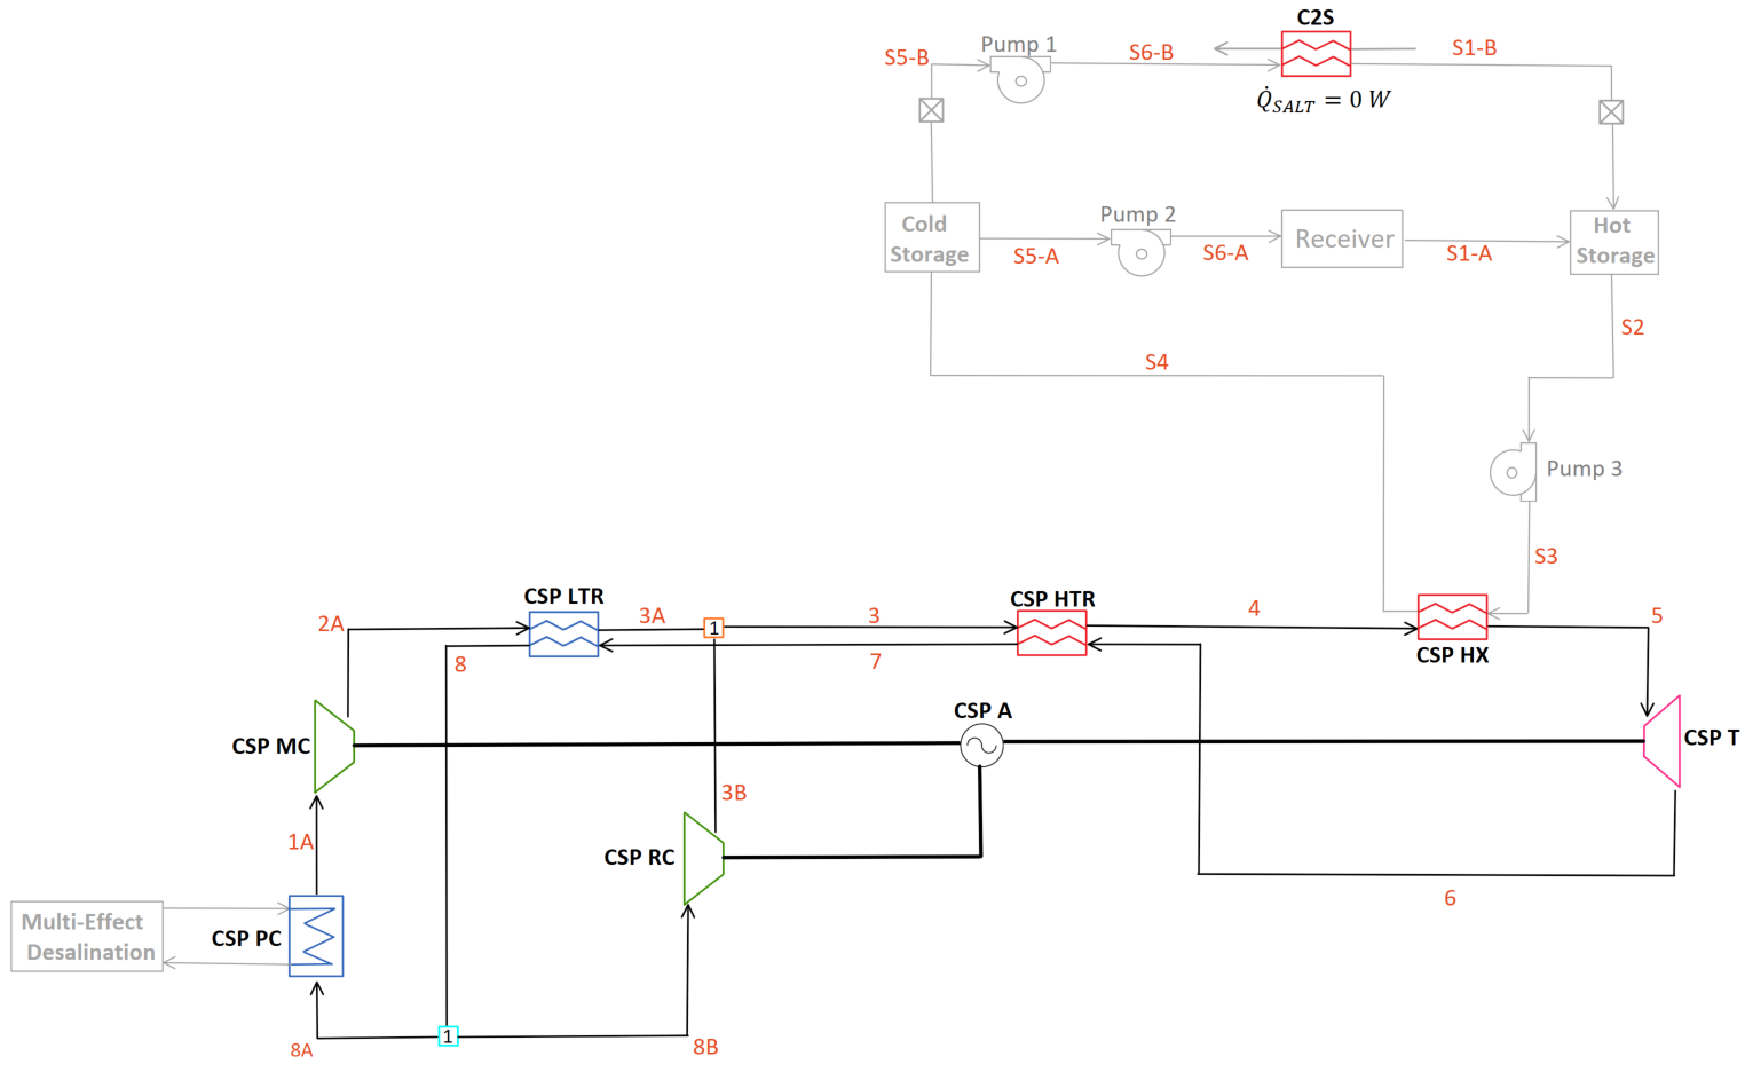
\includegraphics[width=\linewidth]{Definitions/c-csp-on.pdf}
    \caption{Diagram for C-CSP-ON with focus on electricity generation\label{c-csp-on}}
\end{figure}
\begin{paracol}{2}
\linenumbers
\switchcolumn

 Due to the individual operation while the cycles are generating electricity, C-CSP-ON is not directly impacted by the LFR low end temperatures. Instead, a sensitivity study is done on the temperature of the cold TES. Two temperatures are tested, $390^{\circ}$C and $440^{\circ}$C, to observe the impact of cold TES temperature on cycle efficiency. Efficiencies need to be combined to draw a comparison of the two-cycle configurations to the single cycle configurations; C-1HTR1T-ON and C-2HTR3T-ON. Equation \ref{eq-eta-2cycle} is used to calculate this combined two-cycle efficiency.

 \begin{equation}
    \label{eq-eta-2cycle}
    \eta_{combined} = \frac{\dot{W}_{A,C\text{-}LFR\text{-}ON}+\dot{W}_{A,C\text{-}CSP\text{-}ON}}{\dot{Q}_{LFRHX}+\dot{Q}_{CSPHX}},
\end{equation}

Equation \ref{eq-eta-2cycle} is the ratio of total alternator (net) power of C-LFR-ON, $\dot{W}_{A,C\text{-}LFR\text{-}ON}$, and C-CSP-ON, $\dot{W}_{A,C\text{-}CSP\text{-}ON}$, to the total heat input into the cycles from the LFR and CSP heat exchangers, $\dot{Q}_{LFRHX}+\dot{Q}_{CSPHX}$.




\subsubsection{C-1HTR1T-ON} 
%--------------------------------------------------------------------------------------

One drawback of having a two-cycle design, as seen in the C-LFR-ON and C-CSP-ON, is doubling the number of system components. Combining the two cycles into one would reduce redundancy, complexity, and cost. Heat addition from the CSP HX and LFR HX in parallel orientation is therefore studied in the C-1HTR1T-ON model. This model studies what impact mixing different temperature flows prior to the turbine has on cycle efficiency. The diagram for this cycle is illustrated in Figure \ref{c-1htr1t-on}.

\end{paracol}

\begin{figure}[H] 
    \widefigure
    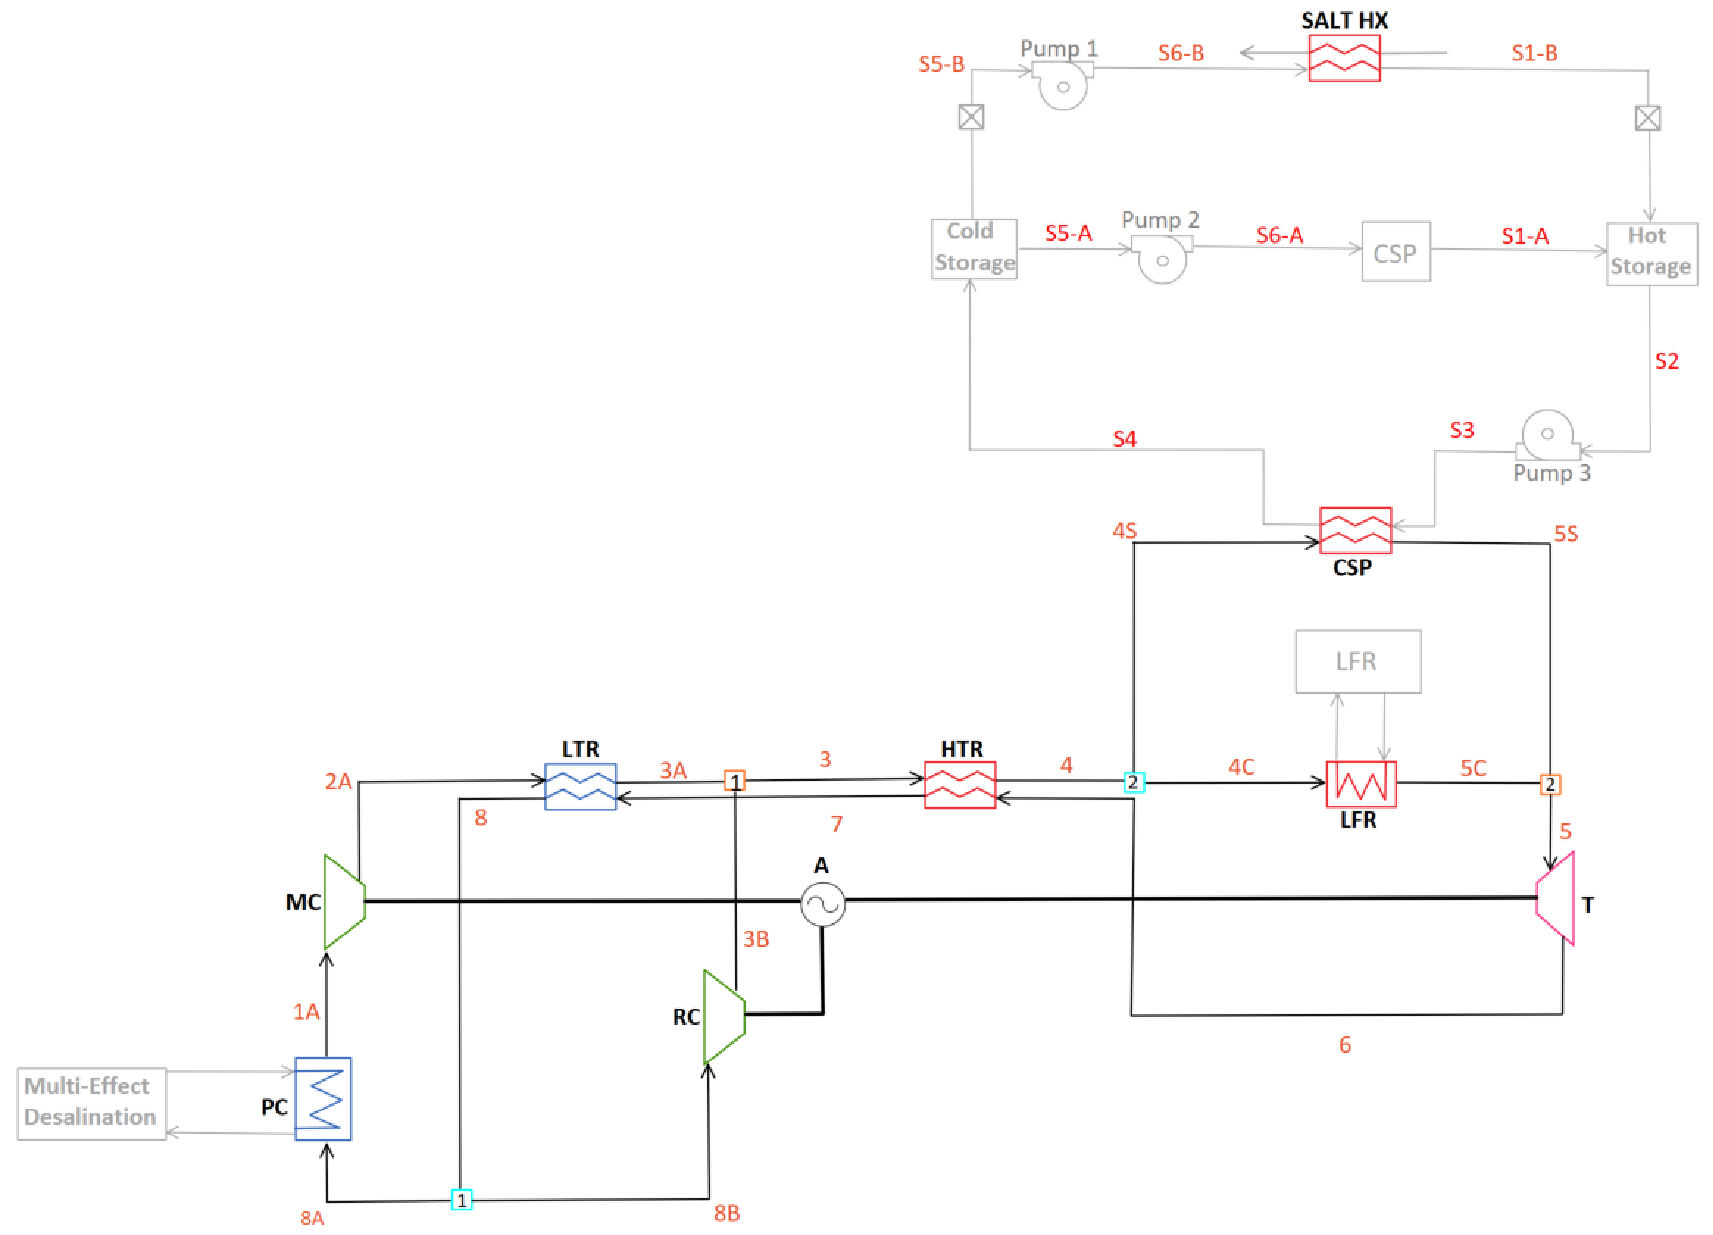
\includegraphics[width=\linewidth]{Definitions/c-1htr1t-on.pdf}
    \caption{Diagram for C-1HTR1T-ON with focus on electricity generation\label{c-1htr1t-on}}
\end{figure}


\begin{paracol}{2}
\linenumbers
\switchcolumn

The C2S is located around the turbine and LFR at state points 5 to 6 depending on the charging cycle configuration: pre, parallel, post or circulator. In the C-1HTR1T-ON cycle, the LFR HX and CSP HX have identical inlet temperatures due to splitting the flow prior to their parallel orientation. Therefore, three sensitivity studies are done on the model. The initial two studies have the low LFR temperature constrained to the value of $400^{\circ}$C with varied cold CSP TES temperature and maximized cycle efficiency. To achieve a maximum cycle efficiency, the split fraction amount of flow to the main compressor, $y_{1}$, is parametrically studied.
Two cold TES temperatures are tested with constrained LFR low temperature of $400^{\circ}$C: 
\begin{itemize}
    \item	$410^{\circ}$C: Lowest cold TES temperature possible due to the sCO$_2$ cold inlet constrained from the LFR to $400^{\circ}$C and the addition of $10^{\circ}$C approach temperature;
    \item	$440^{\circ}$C: Upper bound temperature on cold TES storage;
    \item	$390^{\circ}$C: Unconstrained LFR cold inlet temperature allows a lower cold TES of $390^{\circ}$C to be achieved. This allows for a larger temperature drop across the CSP HX, increasing dispatchability.
\end{itemize}


\subsubsection{C-2HTR3T-ON} 
%--------------------------------------------------------------------------------------

The identical inlet temperatures due to the parallel configuration makes the C-1HTR1T-ON cycle configuration restricted. Another single cycle configuration is desired to allow dissimilar inlet temperatures for the CSP HX and LFR HX while additionally testing the effect that mixing flows downstream from the HTR has on cycle efficiency. 

In practice, sCO$_2$ cycles typically have 3 turbines, with 2 of these driving the compressor and recompressor. Therefore, this configuration will not in general require additional turbines compared to the C-1HTR1T-ON configuration. Furthermore, it is anticipated that the cost of the high temperature recuperator is likely most related to its volume, and hence having two smaller high temperature recuperators is unlikely to cost significantly more than one large one. 

This cycle, C-2HTR3T-ON, can be seen in Figure \ref{c-2htr3t-on} and has two high temperature recuperators and three turbines. The LFR is powering one turbine, T1, and transferring unused heat to the flow entering LFR HX through a dedicated high temperature recuperator, HTR. The cycle with heat addition from the CSP powers the other two turbines, which for modeling purposes are combined into a single turbine T2, while having a dedicated high temperature recuperator, HTR2. The two turbines displayed as T2 can be modeled as a singular turbine because their isentropic efficiencies are identical causing the inlet and outlet conditions of the turbines to be consistent with a singular turbine. Additionally, the power produced by the two turbines is proportional to mass flow rate, each receives a fraction of the mass flow rate therefore producing the same fraction of power. Summing these power fractions together yields the total power of a singular turbine in the same position. After the high temperature recuperators, the two flows are combined and sent to the LTR hot side. 

\end{paracol}
\begin{figure}[H]
    \widefigure
    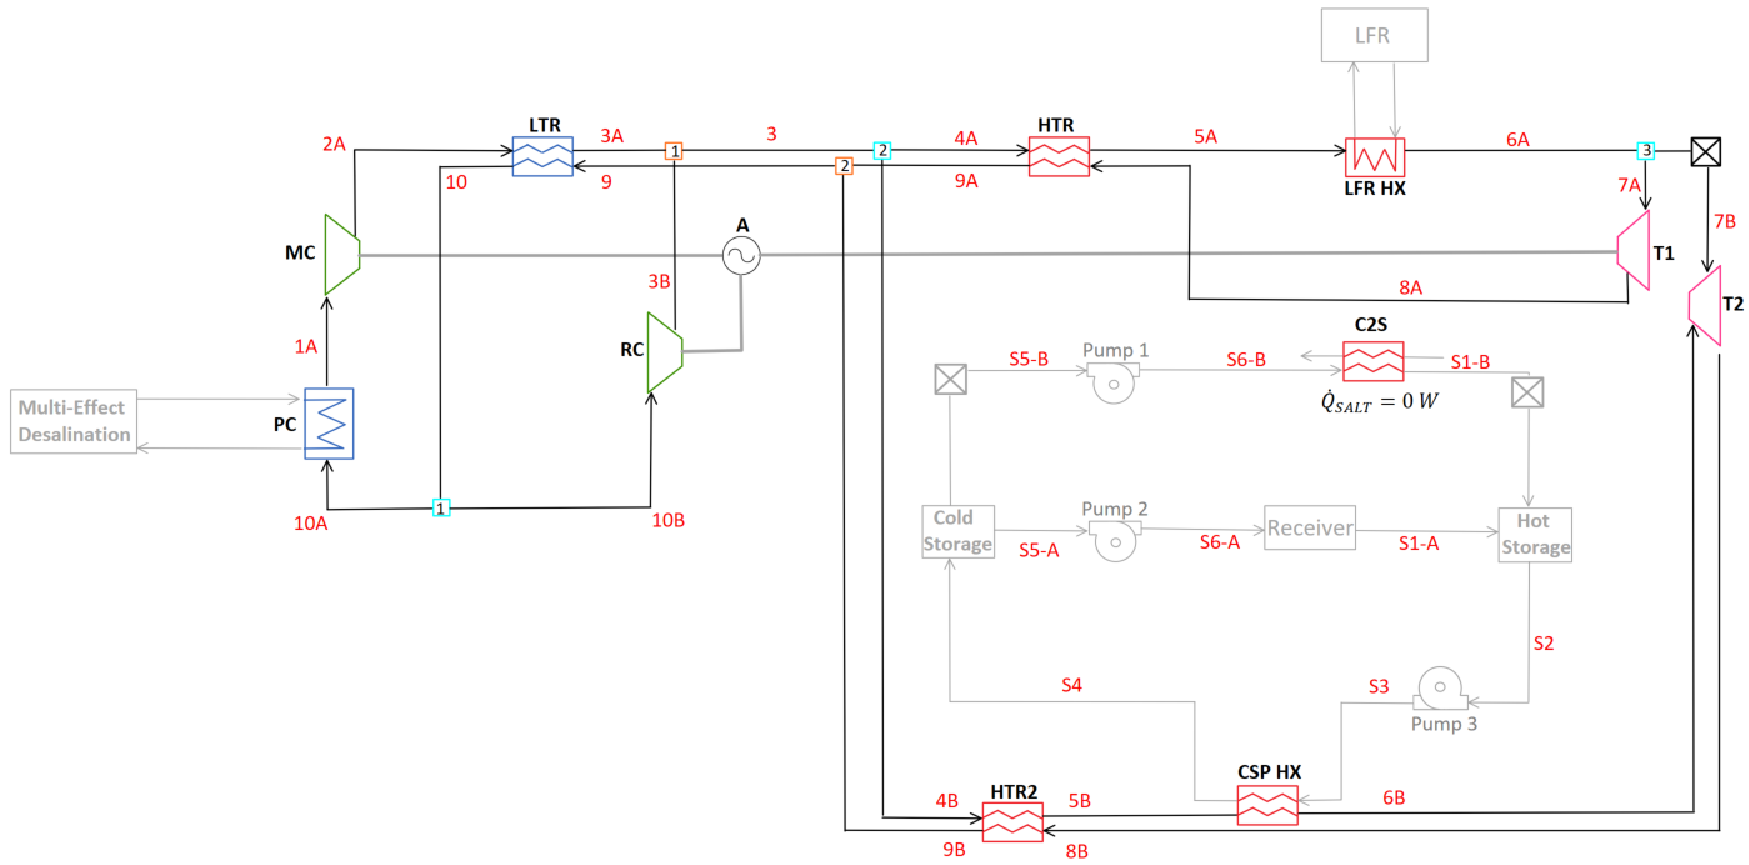
\includegraphics[width=\linewidth]{Definitions/c-2htr3t-on.pdf}
    \caption{Diagram for C-2HTR3T-ON with focus on electricity generation\label{c-2htr3t-on}}
\end{figure}
\begin{paracol}{2}
\linenumbers
\switchcolumn

The C2S heat exchanger is located around the turbine and LFR at 7A to 8A depending on the charging configuration: pre, post, parallel or circulator. Three sensitivity studies are done on the C-2HTR3T-ON model -- two with the LFR low temperature constrained and one without this constraint. The two constrained studies, with an LFR temperature of $400^{\circ}$, have varied cold CSP TES temperature with the lowest temperature of $390^{\circ}$C and highest temperature of $440^{\circ}$C. The unconstrained low LFR inlet study is calculated at a cold CSP TES temperature of $390^{\circ}$C.



\subsection{Thermal Energy Storage Charging Techniques} 
%======================================================================================

Charging cycle configurations accommodate energy storage modes of operation. These configurations examine the location of LFR heat extraction via C2S. To maximize the available heat for extraction, alternator net power is set to zero, therefore requiring the turbine power to balance with the compressors' demand. Despite the components being non-ideal and consuming power, the recompression cycle continues to operate, ensuring that there is mass flow to transfer heat from the Brayton cycle to C2S. The excess energy from the LFR is thermally stored in the TES for later use when grid demand increases. Comparison of the heat extraction point in the cycle, C2S, is accomplished by implementing C2S in different locations around the turbine in the C-LFR-ON non-charging cycle configuration; C-LFR-PRE has the turbine prior to C2S, C-LFR-POST has the turbine after C2S, C-LFR-PAR has the turbine in parallel to C2S, and C-LFR-CIRC uses a circulating loop instead of in-flow implementation. C-LFR-ON is the configuration used for these studies because during charging operation, flow through the CSP HX is deactivated, effectively making all non-charging cycles take the identical form of C-LFR-ON. To quantify the effectiveness of TES charging techniques, Equation \ref{eq-eta-heatstorage} defines the heat storage efficiency, $\eta_{heatstorage}$.  

\begin{equation}
    \label{eq-eta-heatstorage}
    \eta_{heatstorage} = \frac{\dot{Q}_{C2S}}{\dot{Q}_{LFRHX}+\dot{Q}_{CSPHX}},
\end{equation}

In the heat storage efficiency equation, $\dot{Q}_{C2S}$ is the amount of heat transferred through C2S, and the addition of $\dot{Q}_{LFRHX}$ and $\dot{Q}_{CSPHX}$ is the total amount of heat input into the system from the LFR HX and CSP HX. 

\subsubsection{C-LFR-PRE} 
%--------------------------------------------------------------------------------------

The high temperature sCO$_2$ leaving the LFR HX flows through the LFR turbine converting thermal energy to usable work. The outlet temperature of the LFR turbine is at a temperature suitable to charge the hot TES, therefore the flow is passed through C2S exchanging heat to the cold solar salt. The diagram outlining this process is C-LFR-PRE in Fig. \ref{c-lfr-pre}. 

\end{paracol}
\begin{figure}[H]
    \widefigure
    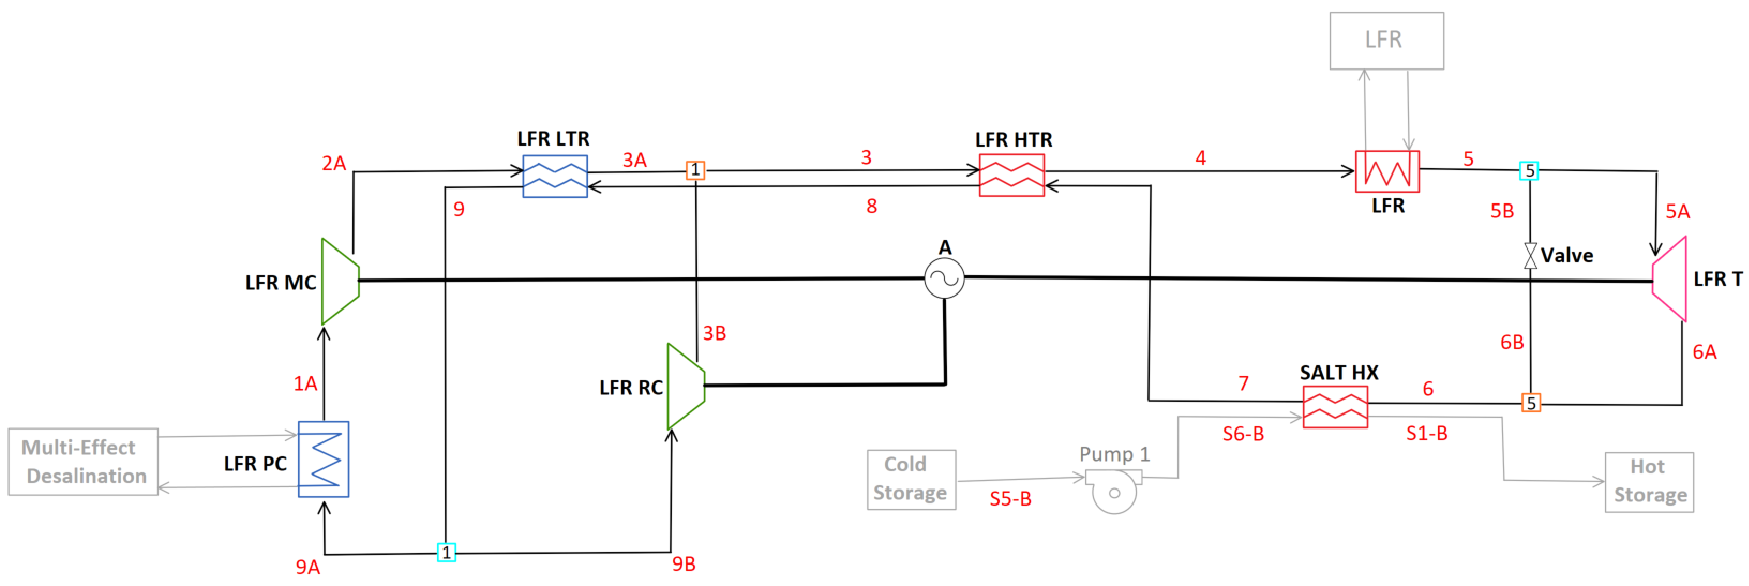
\includegraphics[width=\linewidth]{Definitions/c-lfr-pre.pdf}
    \caption{Diagram for C-LFR-PRE thermal energy storage charging orientation\label{c-lfr-pre}}
\end{figure}
\begin{paracol}{2}
\linenumbers
\switchcolumn

A problem arises with this salt charging configuration. The temperature out of the turbine is not high enough to charge the hot CSP TES to the required value of $560^{\circ}$C when the turbine power is balanced with the compressor demand. To raise the temperature, some of the high temperature flow before the turbine is redirected through a valve and combined after the turbine. Limiting the flow through the turbine reduces the turbine power and compressor power because of the balancing requirement. Due to the reduction in available compressor power, the LFR RC is effectively bypassed, and a large portion of usable heat is expelled in the LFR PC before the LFR MC. The thermal storage efficiency reduces as a result of the large amount of heat rejected in the LFR PC. 



\subsubsection{C-LFR-POST} 
%--------------------------------------------------------------------------------------

Moving the heat extraction prior to the turbine is analyzed in C-LFR-POST. This diagram is seen in Figure \ref{c-lfr-post}.

\end{paracol}
\begin{figure}[H]
    \widefigure
    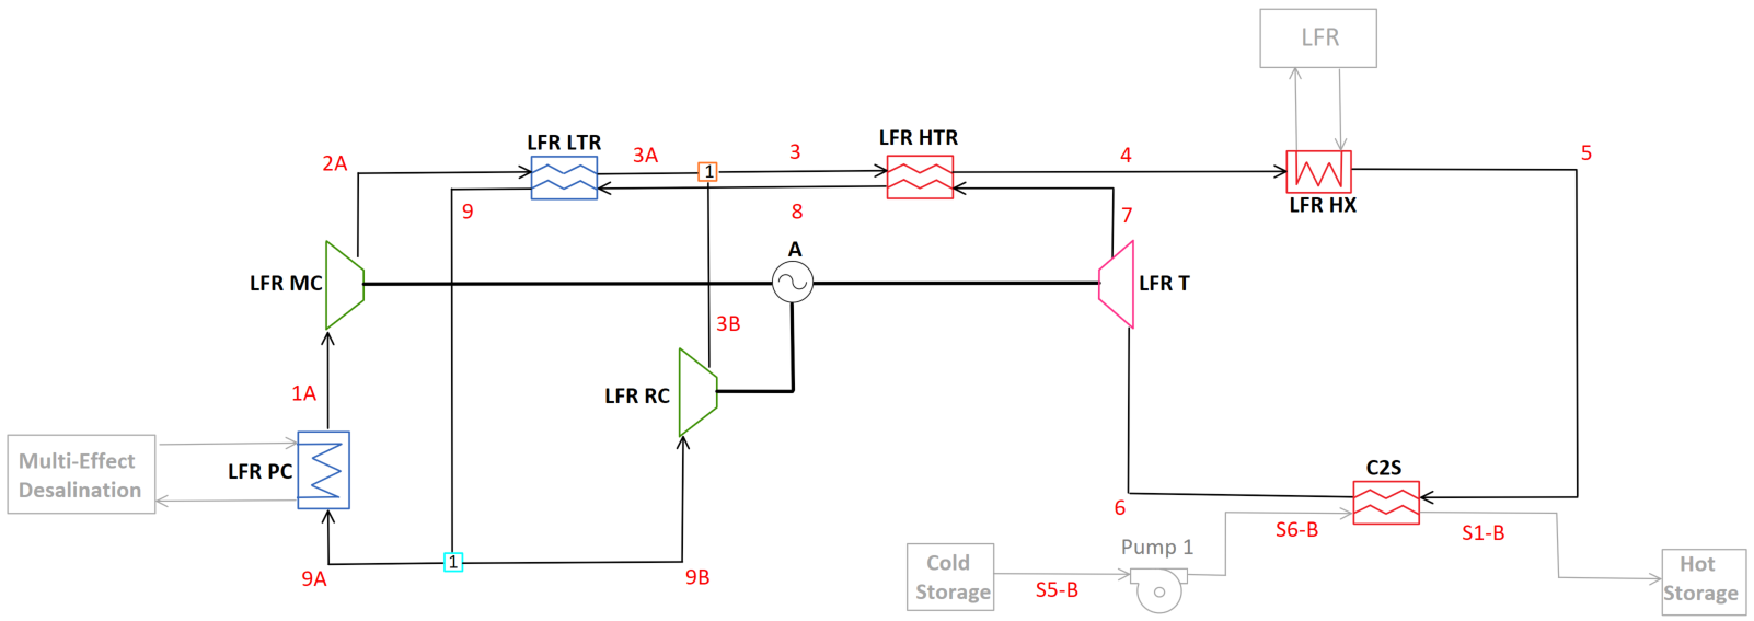
\includegraphics[width=\linewidth]{Definitions/c-lfr-post.pdf}
    \caption{Diagram for C-LFR-POST thermal energy storage charging orientation\label{c-lfr-post}}
\end{figure}
\begin{paracol}{2}
\linenumbers
\switchcolumn

This TES charging cycle extracts heat before the turbine and therefore has a large negative effect on the amount of work that the turbine is producing. The turbine power offsets the requirements of both compressors, requiring the turbine inlet temperature to be high. The amount of energy that is extracted before the turbine is small and therefore the heat storage efficiency is fractional compared to other charging techniques. There is no quantitative study done on this case because, due to the efficiency losses, it is non-viable. 

\subsubsection{C-LFR-PAR} 
%--------------------------------------------------------------------------------------

The requirements of the turbine and CSP hot TES can be satisfied by splitting the flow before the turbine. The flow through the salt heat exchanger in this cycle is therefore separate from the turbine. After the salt heat exchanger, a valve is needed to reduce the pressure, this TES charging cycle is C-LFR-PAR shown in Figure \ref{c-lfr-par}.

A sensitivity study with varying cold CSP TES temperature is carried out to determine the impact on heat storage efficiency. The study considers two temperature values of $390^{\circ}$C and $440^{\circ}$C.

\clearpage
\end{paracol}
\begin{figure}[H]
    \widefigure
    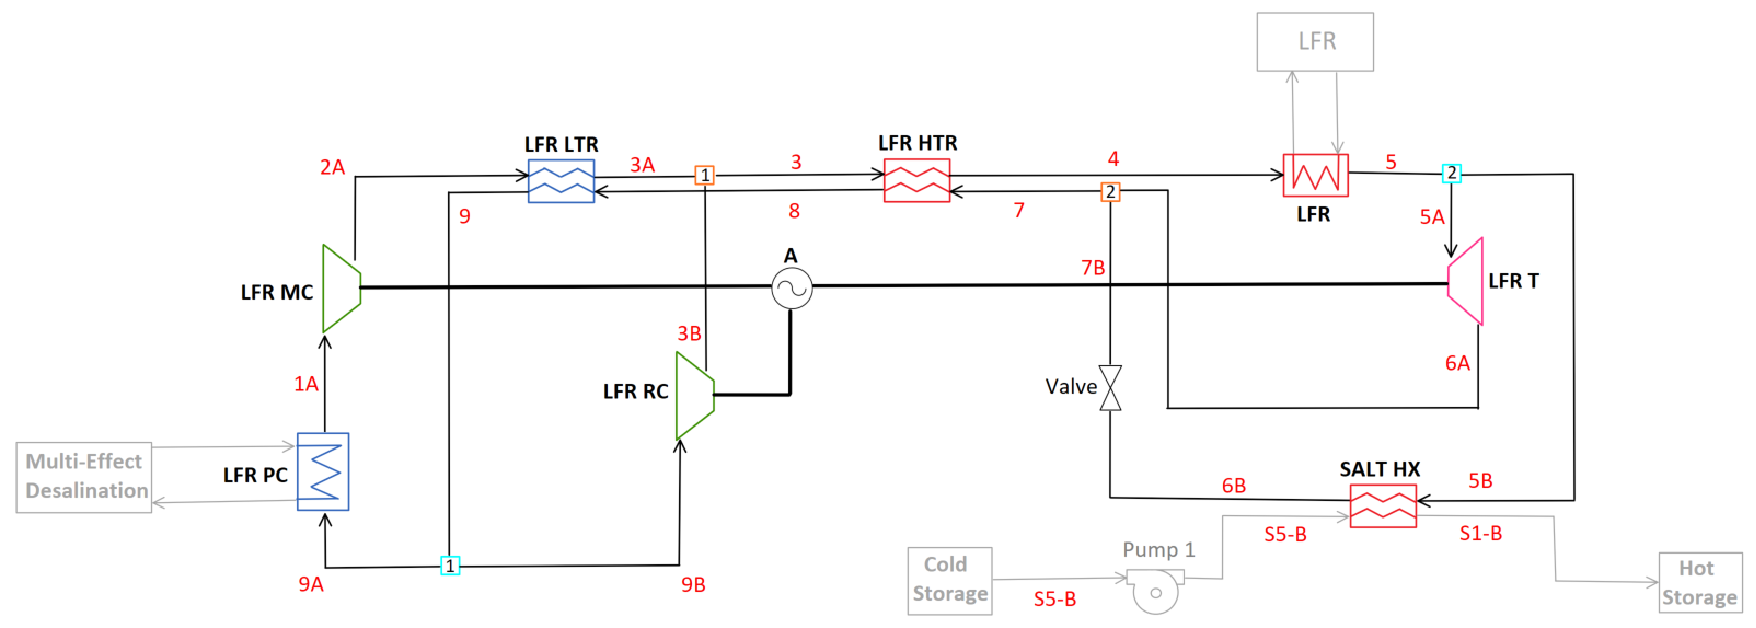
\includegraphics[width=\linewidth]{Definitions/c-lfr-par.pdf}
    \caption{Diagram for C-LFR-PAR thermal energy storage charging orientation\label{c-lfr-par}}
\end{figure}
\begin{paracol}{2}
\linenumbers
\switchcolumn


\subsubsection{C-LFR-CIRC} 
%--------------------------------------------------------------------------------------

The full diagram for C-LFR-CIRC is shown in Figure \ref{c-lfr-circ}.
\end{paracol}
\begin{figure}[H]
    \widefigure
    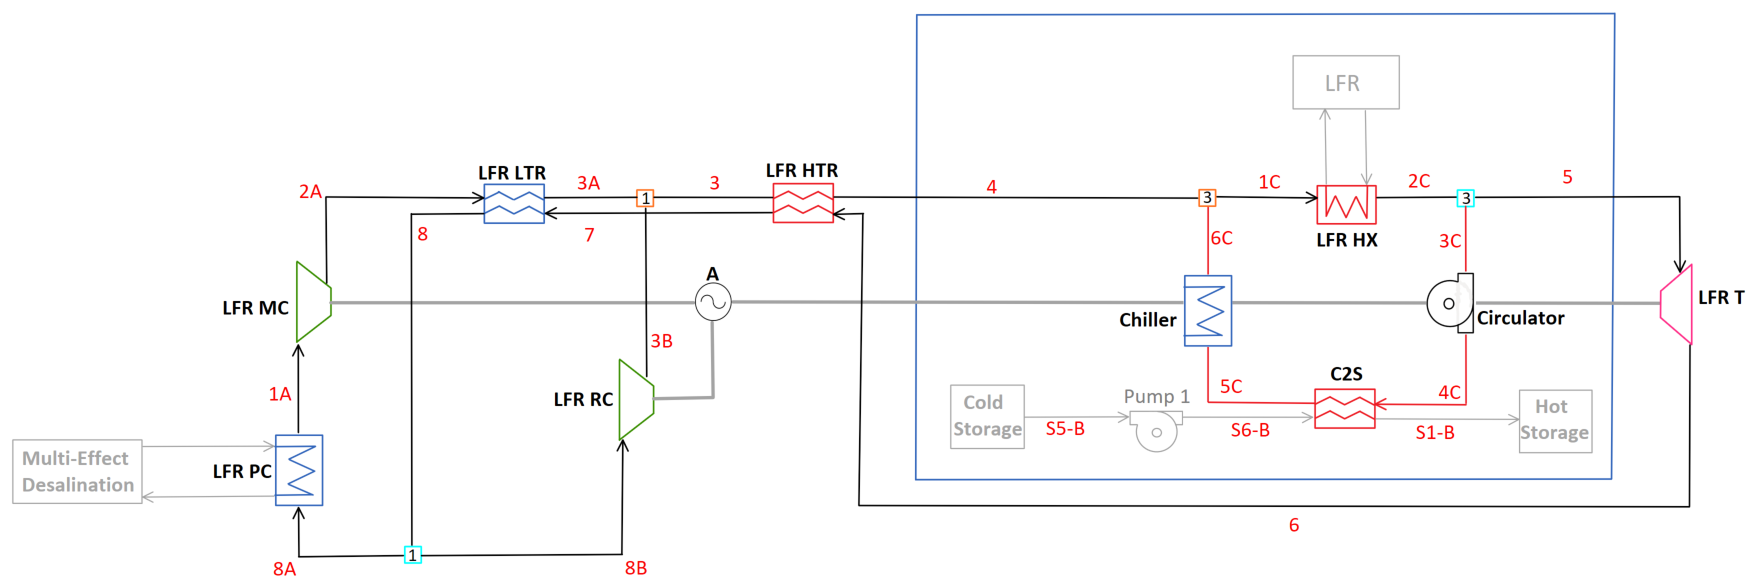
\includegraphics[width=\linewidth]{Definitions/c-lfr-circ.pdf}
    \caption{Full diagram for C-LFR-CIRC thermal energy storage charging orientation\label{c-lfr-circ}}
\end{figure}
\begin{paracol}{2}
\linenumbers
\switchcolumn

The charging subsection of this diagram is composed of a circulation cycle that has heat inputted through the LFR heat exchanger. A separated circulation cycle has a loop which avoids the losses associated with compressor and turbine, therefore achieving higher heat storage efficiency than possible with full cycle operation. This subsection is encircled in blue and can be seen in Figure \ref{c-lfr-circ-sub}.

The flow continues through a circulator which is assumed to have negligible pressure rise (i.e. there is assumed to be negligible pressure drop in this case). A heat exchanger, C2S, extracts heat from the flow, storing the thermal energy in the hot TES for later use. Excess heat that is not extracted is then dumped into a reservoir through the chiller to bring the temperature of the flow down to LFR cool side operating temperature of $400^{\circ}$C. Three different cold TES temperatures; $390^{\circ}$C, $410^{\circ}$C, and $440^{\circ}$C, are compared in a sensitivity study. 

% \end{paracol}
\begin{figure}[H]
    \widefigure
    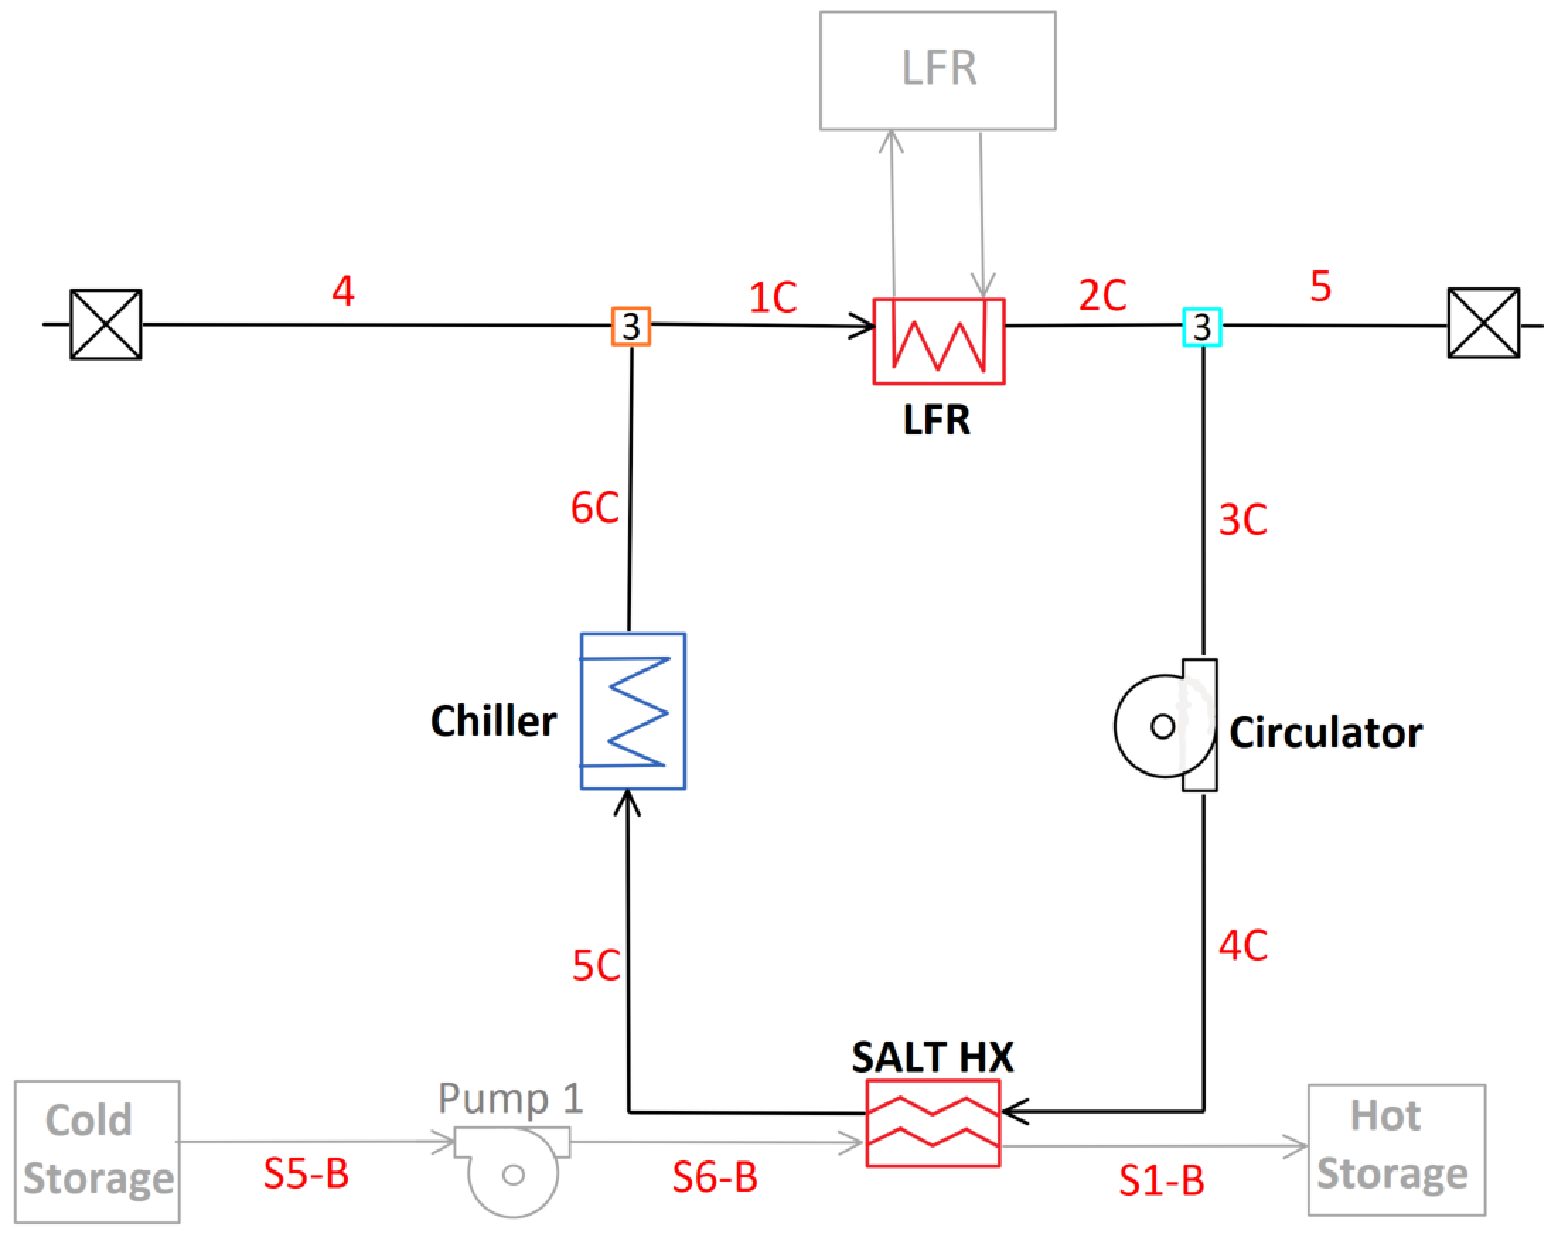
\includegraphics[width=0.7\linewidth]{Definitions/c-lfr-circ-sub.pdf}
    \caption{Diagram for C-LFR-CIRC sub-cycle thermal energy storage charging orientation\label{c-lfr-circ-sub}}
\end{figure}
% \begin{paracol}{2}
% \linenumbers
% \switchcolumn




%%%%%%%%%%%%%%%%%%%%%%%%%%%%%%%%%%%%%%%%%%%%%%%%%%%%%%%%%%%%%%%%%%%%%%%%%%%%%%%%%%%%%%%
\section{Results and Discussion}

For all cycle configurations presented, with constrained or unconstrained LFR low temperature inlet and varied cold TES temperature, cycle and heat storage efficiencies are maximized using parametric studies on flow splitter fractions. These results are obtained using standardized values found in Table \ref{tab-cycle_sum} for a more direct comparison between cycles. Presentation and discussion of the results is fulfilled in the following section. 

\subsection{Non-Charging Cycle Configurations}
%======================================================================================

The three non-charging cycle models have a focus on producing the highest positive alternator power to heat input, or cycle efficiency. The two-cycle configuration, composed of C-LFR-ON and C-CSP-ON, has independent recompression cycles with dedicated compressors, turbine, recuperators, and pre-cooler for the LFR and CSP. C-1HTR1T-ON, with the heat additions in parallel, and C-2HTR3T, with dedicated HTR for both heat additions, are cycles which incorporate the CSP and LFR in the same cycle. The results from studies done on these cycles are displayed in Table \ref{tab-noncharg}. 

The calculated values reported in Table \ref{tab-noncharg} are component power, mass flow fractions, and counter-flow heat exchanger specifications. Columns labeled with '$C$' headers have the LFR sCO$_2$ low inlet temperature constrained to 400$^{\circ}$C while those labeled with '$U$' are unconstrained and calculated based off of a parametric study on the MC mass flow fraction. Values listed in the Cold TES Temperature row are set to values of 390$^{\circ}$C, 410$^{\circ}$C, or 440$^{\circ}$C to study the effects that cold TES temperature has on cycle efficiency and to accommodate certain characteristics of cycle configurations. Cycles that do not contain the listed component and omit the associated values. 
\clearpage 
% \mw{Check that the column breakdown and grouping is correct in what I've changed.}
\end{paracol}
\begin{specialtable}[H] 
    %[htbp]
    
    \caption{Calculated system parameters for non-charging cycle configurations with constrained (\textit{C}) and unconstrained (\textit{U}) lead-cooled fast reactor low-end temperature.\label{tab-noncharg}}
    \resizebox{\columnwidth}{!}{
    \begin{tabular}{lc|cc|cc|ccc|ccc}
    \toprule
     &  & \multicolumn{2}{c|}{\textbf{C-LFR-ON}} & \multicolumn{2}{c|}{\textbf{C-CSP-ON}}  &	\multicolumn{3}{c|}{\textbf{C-1HTR1T-ON}}	&	\multicolumn{3}{c}{\textbf{C-2HTR3T-ON}} \\
    \textbf{Definition} & \textbf{Variable} & \textit{U} & \textit{C} & \textit{N/A} & \textit{N/A} &	\textit{U}	&	\textit{C}	&	\textit{C}	&	\textit{U}	&	\textit{C}	&	\textit{C}
    \\
    \midrule
    Cycle Efficiency (\%)	&	$\eta_{cycle}$	&	47.08	&	45.28	&	45.58	&	45.93	&	44.9	&	44.22	&	44.22	&	46.10	&	44.34	&	44.35	\\
    LFR Inlet Temperature ($^{\circ}$C)	&	$T_{4,4C,5A}$	&	415.1	&	400	&	$\cdot$	&	$\cdot$	&	380	&	400	&	400	&	415.2	&	400	&	400	\\
    Cold TES Temperature ($^{\circ}$C)	&	$T_{CS}$	&	$\cdot$	&	$\cdot$	&	390	&	440	&	390	&	410	&	440	&	390	&	390	&	440	\\
    Alternator Power (MW)	&	$\dot{W}_{A}$	&	447.3	&	430.2	&	339.1	&	340.6	&	763.9	&	752.3	&	752.6	&	783.7	&	753.7	&	754	\\
    PC Heat Transfer (MW)	&	$\dot{Q}_{PC}$	&	502.7	&	519.8	&	418.5	&	420.2	&	937.4	&	949.2	&	949.3	&	917.6	&	947.6	&	947.9	\\
    MC Power (MW)	&	$\dot{W}_{MC}$	&	115	&	118.9	&	95.73	&	96.13	&	214.5	&	194.8	&	194.8	&	209.9	&	216.8	&	216.9	\\
    RC Power (MW)	&	$\dot{W}_{RC}$	&	116.6	&	77.3	&	97.22	&	97.71	&	217.4	&	285.7	&	285.7	&	213.5	&	140.8	&	140.8	\\
    T1 Power (MW)	&	$\dot{W}_{T1}$	&	678.9	&	626.4	&	532.1	&	534.5	&	1196	&	1233	&	1233	&	679.3	&	626.3	&	626.3	\\
    T2 Power (MW)	&	$\dot{W}_{T2}$	&	$\cdot$	&	$\cdot$	&	$\cdot$	&	$\cdot$	&	$\cdot$	&	$\cdot$	&	$\cdot$	&	527.8	&	485	&	485.4	\\
    MC Mass Flow Fraction (-)	&	$y_{1}$	&	0.7	&	0.7844	&	0.6996	&	0.6994	&	0.7	&	0.6333	&	0.6333	&	0.6993	&	0.7846	&	0.7846	\\
    LFR Mass Flow Fraction (-)	&	$y_{2}$	&	$\cdot$	&	$\cdot$	&	$\cdot$	&	$\cdot$	&	0.4485	&	0.4928	&	0.4929	&	0.5478	&	0.5486	&	0.5484	\\
    LTR UA Value (MW/$^{\circ}$C)	&	$UA_{LTR}$	&	54.68	&	22.84	&	45.4	&	45.53	&	102	&	91.63	&	91.64	&	134.4	&	41.56	&	41.57	\\
    LTR Capacitance Ratio (-)	&	$CR_{LTR}$	&	0.9867	&	0.8473	&	0.9858	&	0.9854	&	0.9867	&	0.9066	&	0.9066	&	0.9853	&	0.847	&	0.847	\\
    LTR Heat Transfer Rate (MW)	&	$\dot{Q}_{LTR}$	&	656.8	&	366.5	&	548.3	&	551.4	&	549.2	&	614.9	&	615.1	&	1204	&	667.1	&	667.3	\\
    LTR Effectiveness (-)	&	$\varepsilon_{LTR}$	&	0.92	&	0.8742	&	0.9201	&	0.9202	&	0.92	&	0.9485	&	0.9485	&	0.9414	&	0.8741	&	0.8741	\\
    HTR UA Value (MW/$^{\circ}$C)	&	$UA_{HTR}$	&	48.29	&	42.71	&	34.58	&	34.72	&	78.22	&	82.3	&	82.34	&	48.32	&	42.69	&	42.69	\\
    HTR Capacitance Ratio (-)	&	$CR_{HTR}$	&	0.8657	&	0.8143	&	0.8593	&	0.8594	&	0.8595	&	0.8754	&	0.8755	&	0.8661	&	0.8142	&	0.8142	\\
    HTR Heat Transfer Rate (MW)	&	$\dot{Q}_{HTR}$	&	998.1	&	1161	&	665.4	&	667.7	&	679.2	&	742.6	&	743	&	545.7	&	636.8	&	636.6	\\
    HTR Effectiveness (-)	&	$\varepsilon_{HTR}$	&	0.9544	&	0.9627	&	0.9436	&	0.9436	&	0.9445	&	0.9441	&	0.9441	&	0.9542	&	0.9627	&	0.9627	\\
    HTR2 UA Value (MW/$^{\circ}$C)	&	$UA_{HTR2}$	&	$\cdot$	&	$\cdot$	&	$\cdot$	&	$\cdot$	&	$\cdot$	&	$\cdot$	&	$\cdot$	&	34.29	&	31.61	&	31.63	\\
    HTR2 Capacitance Ratio (-)	&	$CR_{HTR2}$	&	$\cdot$	&	$\cdot$	&	$\cdot$	&	$\cdot$	&	$\cdot$	&	$\cdot$	&	$\cdot$	&	0.8594	&	0.8074	&	0.8074	\\
    HTR2 Heat Transfer Rate (MW)	&	$\dot{Q}_{HTR2}$	&	$\cdot$	&	$\cdot$	&	$\cdot$	&	$\cdot$	&	$\cdot$	&	$\cdot$	&	$\cdot$	&	298.1	&	363.4	&	363.8	\\
    HTR2 Effectiveness (-)	&	$\varepsilon_{HTR2}$	&	$\cdot$	&	$\cdot$	&	$\cdot$	&	$\cdot$	&	$\cdot$	&	$\cdot$	&	$\cdot$	&	0.9436	&	0.9561	&	0.9561	\\
    CSPHX UA Value (MW/$^{\circ}$C)	&	$UA_{CSPHX}$	&	$\cdot$	&	$\cdot$	&	71.34	&	26.92	&	33.72	&	73.4	&	35.05	&	70.88	&	44.92	&	23.13	\\
    CSPHX Capacitance Ratio (-)	&	$CR_{CSPHX}$	&	$\cdot$	&	$\cdot$	&	0.9924	&	0.701	&	0.8104	&	0.9957	&	0.8034	&	0.9926	&	0.9138	&	0.6454	\\
    CSPHX Heat Transfer Rate (MW)	&	$\dot{Q}_{CSPHX}$	&	$\cdot$	&	$\cdot$	&	757.6	&	760.8	&	751.3	&	751.5	&	751.9	&	751.3	&	751.3	&	751.9	\\
    CSPHX Effectiveness (-)	&	$\varepsilon_{CSPHX}$	&	$\cdot$	&	$\cdot$	&	0.945	&	0.945	&	0.945	&	0.9381	&	0.9374	&	0.9450	&	0.9493	&	0.9493	\\
    \bottomrule
    \end{tabular}
    }
\end{specialtable}
\begin{paracol}{2}
\linenumbers
\switchcolumn


\subsubsection{Two-Cycle Configuration: C-LFR-ON and C-CSP-ON}

The two-cycle configuration has the CSP and LFR operating in separate recompression cycles when the focus is on electrical generation, therefore these two cycles are analyzed individually. C-LFR-ON has the highest efficiency during unconstrained operation with a gain of 1.8 percentage points. The unconstrained case allows for smaller temperature gradient across the LFR, an increase in recuperator effectiveness, and an increase in recuperator capacitance ratio, all of which reduce sources of irreversibility in the cycle \cite{klein_nellis_2011}. Increasing the LFR sCO$_2$ inlet temperature above the design value of $400^{\circ}$C is favorable from a cycle efficiency perspective, but reduces the LFR thermal power. This is because the LFR mass flow rate and outlet temperature are constrained by materials properties (to limit creep, corrosion and erosion), so a lower inlet temperature implies a lower thermal power. In principle, dropping the LFR inlet temperature further, to as low as $340^{\circ}$C (beyond which lead freezing becomes limiting), would further increase thermal power at the expense of cycle efficiency, so a trade-off is needed. When unconstrained, the sCO$_2$ inlet temperature to the LFR increases by $15.1^{\circ}$C to a value of $415.1^{\circ}$C, increasing LFR efficiency but demanding a larger, more idealized, LFR heat exchanger.

C-CSP-ON is not affected by constrained or unconstrained LFR sCO$_2$ inlet temperature because C2S is turned off and therefore the two cycles are not tethered during non-charging configuration. Two individual studies are conducted on the C-CSP-ON cycle cold TES temperature, one with a lower design value of $390^{\circ}$C and another with a higher value of $440^{\circ}$C. A cold TES temperature of $410^{\circ}$C is excluded since it can be presumed to have an efficiency intermediate to the $390^{\circ}$C and $440^{\circ}$C calculated values. Cold TES temperature is found to have a negligible effect on cycle efficiency between the two studied cases, with the $440^{\circ}$C case gaining 0.35 percentage points. The component that has the largest change in values is the CSP HX with a large drop in capacitance ratio and UA value, therefore the lower temperature of $390^{\circ}$C for cold TES temperature is ideal increasing the performances of the heat exchanger. 

Combining the two-cycle efficiencies using Equation \ref{eq-eta-2cycle} gives a more direct comparison to the single cycle configurations; C-1HTR1T and C-2HTR3T. Two combined efficiencies are calculated for the two-cycle configuration combination. The first has the highest efficiency, combining the unconstrained C-LFR-ON LFR low temperature and C-CSP-ON $440^{\circ}$C cold TES cases. This combined efficiency yields a value of 46.1\% (which is almost identical to the efficiency achieved by C-2HTR3T-ON shown in Table \ref{tab-noncharg}). The second combined configuration has a lower efficiency with favorable LFR characteristics and solar salt mass flow rate. This combination has the constrained C-LFR-ON LFR low temperature and C-CSP-ON $390^{\circ}$C cold TES cases with a combined efficiency of 45.1\%. 


\subsubsection{C-1HTR1T-ON}
The single cycle configuration, C-1HTR1T-ON, has the CSP and LFR heat additions in parallel causing identical inlet conditions. Due to the $10^{\circ}$C approach temperature, the identical inlet conditions lead to a lower bound of $410^{\circ}$C on the cold TES temperature when the sCO$_2$ LFR inlet temperature is constrained to $400^{\circ}$C. A supplementary $440^{\circ}$C cold TES study is run to test the effects that higher temperature storage has on cycle efficiency. Raising the temperature of the cold TES from $410^{\circ}$C to $440^{\circ}$C has no effect on cycle efficiency but did raise the solar salt mass flow rate to accommodate for the lower temperature difference across the CSP HX hot side. Increasing the solar salt mass flow rate requires more storage for the same CSP heat input, a reduction in dispatchability, and larger pumps, increasing the cost of the system. Therefore, a lower cold TES temperature is desirable. Without the constraint on the sCO$_2$ LFR inlet temperature, a study is additionally conducted with cold TES temperature set to $390^{\circ}$C. Of these three sensitivity studies, the cycle that yielded the highest efficiency is the unconstrained, $390^{\circ}$C cold TES with an efficiency gain of 0.68 percentage points over the constrained cases. The high temperature difference between the hot and cold TES reduces the mass flow rate of solar salt and subsequent cost of system components. The sCO$_2$ LFR inlet temperature for the $390^{\circ}$C cold TES study is $380^{\circ}$C, which increases the performance of the LFR heat exchanger as well as allowing for a higher core power. 

\subsubsection{C-2HTR3T-ON}
C-2HTR3T-ON has dedicated recuperators and turbines for the LFR and CSP, allowing for independent inlet temperatures. Three studies are conducted on this cycle with two being constrained and one unconstrained sCO$_2$ LFR inlet conditions. The constrained studies have cold TES temperatures of $390^{\circ}$C and $440^{\circ}$, both of which have negligible efficiency differences. Similarly to the studies done on C-1HTR1T-ON, the $440^{\circ}$C cold TES temperature case has a larger mass flow rate of solar salt and therefore increases component cost. The $390^{\circ}$C unconstrained study has the highest efficiency with a value of 46.10\%, 1.76 percentage points more than the constrained cases. Additionally, the sCO$_2$ LFR inlet temperature is $415.2^{\circ}$C, $15.2^{\circ}$C more than constrained cases, causing heat exchanger parameters to be less than ideal but increasing LFR efficiency.

\subsection{Thermal Energy Storage Charging Techniques}

When the focus of the cycles is thermal storage for later use, the LFR charges the hot TES through the C2S heat exchanger. Studies done on the charging techniques have constrained sCO$_2$ LFR inlet temperatures to $400^{\circ}$C with set values of cold TES temperature of $390^{\circ}$C, $410^{\circ}$C, or $440^{\circ}$C. The two charging techniques which run the full recompression cycle are C-LFR-PRE, with the turbine before the heat extraction, and C-LFR-PAR, with heat extraction in parallel to the turbine. The third charging technique, C-LFR-CIRC, has a dedicated circulation loop and additional chiller and circulator pump to avoid losses associated with the compressors and turbines. The results are presented in Table \ref{tab-charg}.  


% \end{paracol}

\begin{specialtable}[H]  
    %[htbp]
    \caption{Calculated system parameters for charging cycle configurations with constrained (\textit{C}) and unconstrained (\textit{U}) lead-cooled fast reactor low-end temperature.\label{tab-charg}}
    \resizebox{\columnwidth}{!}{
        \begin{tabular}{lc|c|cc|ccc}
            \toprule
            &  & \textbf{C-LFR-PRE} & \multicolumn{2}{c|}{\textbf{C-LFR-PAR}}  &	\multicolumn{3}{c}{\textbf{C-LFR-CIRC}} \\
            \textbf{Definition} & \textbf{Variable} & \textit{C} & \textit{C} & \textit{C} & \textit{C} &	\textit{C}	&	\textit{C}\\
            \midrule
            Cold TES Temperature ($^{\circ}$C)	&	$T_{CS}$	&	390	&	390	&	440	&	390	&	410	&	440	\\
            LFR Inlet Temperature ($^{\circ}$C)	&	$T_{4,1C}$	&	400	&	400	&	400	&	400	&	400	&	400	\\
            Heat Storage Efficiency (\%)	&	$\eta_{heatstorage}$	&	34.53	&	45.30	&	45.30	&	99.92	&	89.66	&	74.29	\\
            Alternator Power (MW)	&	$\dot{W}_{A}$	&	0	&	0	&	0	&	$\cdot$	&	$\cdot$	&	$\cdot$	\\
            PC Heat Transfer (MW)	&	$\dot{Q}_{PC}$	&	622	&	519.6	&	519.6	&	$\cdot$	&	$\cdot$	&	$\cdot$	\\
            MC Power (MW)	&	$\dot{W}_{MC}$	&	142.3	&	118.9	&	118.9	&	$\cdot$	&	$\cdot$	&	$\cdot$	\\
            RC Power (MW)	&	$\dot{W}_{RC}$	&	21.89	&	77.28	&	77.28	&	$\cdot$	&	$\cdot$	&	$\cdot$	\\
            Turbine Power (MW)	&	$\dot{W}_{T}$	&	164.2	&	196.2	&	196.2	&	$\cdot$	&	$\cdot$	&	$\cdot$	\\
            Chiller Heat Transfer (MW)	&	$\dot{Q}_{chill}$	&	$\cdot$	&	$\cdot$	&	$\cdot$	&	0.7245	&	98.25	&	244.2	\\
            MC Mass Flow Fraction (-)	&	$y_{1}$	&	0.9389	&	0.7844	&	0.7844	&	$\cdot$	&	$\cdot$	&	$\cdot$	\\
            C2S Mass Flow Fraction (-)	&	$y_{2}$	&	$\cdot$	&	0.6867	&	0.6867	&	$\cdot$	&	$\cdot$	&	$\cdot$	\\
            Valve Mass Flow Fraction (-)	&	$y_{5}$	&	0.7378	&	$\cdot$	&	$\cdot$	&	$\cdot$	&	$\cdot$	&	$\cdot$	\\
            LTR UA Value (MW/$^{\circ}$C)	&	$UA_{LTR}$	&	6.99	&	22.83	&	22.83	&	$\cdot$	&	$\cdot$	&	$\cdot$	\\
            LTR Capacitance Ratio (-)	&	$CR_{LTR}$	&	0.6754	&	0.8473	&	0.8743	&	$\cdot$	&	$\cdot$	&	$\cdot$	\\
            LTR Heat Transfer Rate (MW)	&	$\dot{Q}_{LTR}$	&	93.05	&	366.4	&	366.4	&	$\cdot$	&	$\cdot$	&	$\cdot$	\\
            LTR Effectiveness (-)	&	$\varepsilon_{LTR}$	&	0.6384	&	0.8742	&	0.8742	&	$\cdot$	&	$\cdot$	&	$\cdot$	\\
            HTR UA Value (MW/$^{\circ}$C)	&	$UA_{HTR}$	&	41.69	&	42.69	&	42.69	&	$\cdot$	&	$\cdot$	&	$\cdot$	\\
            HTR Capacitance Ratio (-)	&	$CR_{HTR}$	&	0.7531	&	0.8143	&	0.8143	&	$\cdot$	&	$\cdot$	&	$\cdot$	\\
            HTR Heat Transfer Rate (MW)	&	$\dot{Q}_{HTR}$	&	1567	&	1160	&	1160	&	$\cdot$	&	$\cdot$	&	$\cdot$	\\
            HTR Effectiveness (-)	&	$\varepsilon_{HTR}$	&	0.9695	&	0.9627	&	0.9627	&	$\cdot$	&	$\cdot$	&	$\cdot$	\\
            C2S UA Value (MW/$^{\circ}$C)	&	$UA_{C2S}$	&	9.04	&	8.037	&	14.24	&	48.29	&	43.16	&	35.63	\\
            C2S Capacitance Ratio (-)	&	$CR_{C2S}$	&	0.4735	&	0.7556	&	0.9339	&	0.8755	&	0.8599	&	0.8294	\\
            C2S Heat Transfer Rate (MW)	&	$\dot{Q}_{C2S}$	&	328	&	430.4	&	430.4	&	949.3	&	851.8	&	705.8	\\
            C2S Effectiveness (-)	&	$\varepsilon_{C2S}$	&	0.9368	&	0.8275	&	0.8307	&	0.9511	&	0.9459	&	0.9355	\\
            C2S Approach Temperature ($^{\circ}$C)	&	$\delta_{C2S}$	&	10	&	35	&	26.27	&	10	&	10	&	10	\\
            \bottomrule
        \end{tabular}
        }
    \end{specialtable}
    % \begin{paracol}{2}
        % \linenumbers
        % \switchcolumn
        
\subsubsection{C-LFR-PRE}
The TES charging technique with the turbine prior to the C2S heat exchanger, C-LFR-PRE, requires the temperature of the C2S inlet to be high enough to charge the hot TES. The hot TES is at a temperature of 560$^{\circ}$C, with a 10$^{\circ}$C approach temperature, therefore the inlet temperature to C2S is required to be at least 570$^{\circ}$C. In cases where the turbine outlet temperature is less than 570$^{\circ}$C, a isenthalpic valve bypasses flow from the high temperature turbine inlet and mixes with the low temperature turbine outlet raising the temperature prior to the C2S heat exchanger. For the C-LFR-PRE configuration to be viable, it requires a larger temperature than the set LFR HX outlet temperature of 595$^{\circ}$C. With this low of a LFR outlet temperature, 73.78\% of the flow is redirected around the turbine to raise the temperature prior to C2S. As the temperature of the hot TES is raised above a value of 540$^{\circ}$C, the amount of flow around the turbine approaches 100\% and balancing the turbine power to compressor power is infeasible. The temperature in the hot TES is therefore set to a lower value of 540$^{\circ}$C to allow for operation of this cycle. With heat storage efficiency maximized, 93.89\% of the flow is sent to the main compressor, rejecting 622 MW of heat out of the cycle through the precooler. This amount of rejected heat is reflected in a heat storage efficiency of 34.53\%, the lowest of all tested TES charging configurations.

\subsubsection{C-LFR-PAR}

To test the effects of splitting flow prior to the turbine, a parallel configuration C-LFR-PAR is studied. To reduce the pressure from 28.8 MPa to 8.8 MPa, an isenthalpic valve is required after heat is extracted for storage through C2S. With this configuration two different values for cold TES are studied, one with a cold TES storage of $390^{\circ}$C the other with a temperature of $440^{\circ}$C. A noteworthy difference for this cycle is the C2S approach temperature is not set to $10^{\circ}$C. Defining the approach temperature as $10^{\circ}$C causes the energy balance governing combiner 2 to be over constrained. Therefore this value is free and calculated to be $35^{\circ}$C for the $390^{\circ}$C case and $26.27^{\circ}$C for the $440^{\circ}$C case. Both of these different temperature cold TES studies do not change the cycle parameters because, as seen in C-1HTR1T-ON and C-2HTR3T-ON, the solar salt mass flow rate adjusts to accommodate for the temperature difference. The higher cold TES temperature of $440^{\circ}$C causes the mass flow rate in the CSP to increase by approximately 650 kg/s. Increasing the mass flow rate has a higher demand on system components but in this situation it allows for the salt to be charged at a higher rate, increasing the storage capabilities. Both cycles have a heat storage efficiency of 45.30\%.

\subsubsection{C-LFR-CIRC}

C-LFR-CIRC is a thermal energy storage charging technique which does not suffer from significant losses associated with turbines, compressors, and heat exchangers. The separate recirculation cycle is modeled extracting heat directly from the LFR, passes the high temperature mass flow through a circulator, exchanges the heat into the hot TES through C2S, then removes heat in a chiller to bring the temperature of the flow down to the inlet temperature of the LFR, ideally $400^{\circ}$C. This is the most adoptable TES charging technique with a wide range of possible TES charging temperatures while transferring a majority of the heat from the LFR into the hot TES. Multiple temperatures for the cold TES are studied; $390^{\circ}$C, $410^{\circ}$C, and $440^{\circ}$C. Of these three temperatures, the highest efficiency is a cold TES temperature of $390^{\circ}$ with a heat storage efficiency of 100\% (not accounting for pressure drop losses, which will be small). The heat storage efficiency reduces as the temperature of the cold TES is increased; the $410^{\circ}$C case has an efficiency of 90\% while the $440^{\circ}$C case has an efficiency of 74\%. This reduction in efficiency is due to the inlet temperature condition on the LFR, the higher the temperature of the cold TES the higher the temperature of the C2S outlet and therefore more heat is being extracted through the chiller to bring the flow temperature down to the LFR inlet temperature. 

There is an interaction between the temperatures selected here and the non-charging cycle configuration. For C-LFR-CIRC, the highest efficiencies are achieved when the cold TES temperature is $10^{\circ}$C less than the inlet to the LFR, this is due to the approach temperature on the C2S heat exchanger. If the sCO$_2$ LFR inlet temperature is constrained to $400^{\circ}$C, then the desired cold TES temperature is $390^{\circ}$C to allow for the apporach temperature. If the cold TES is at a higher temperature, then the chiller is needed. This then implies that the sCO$_2$ inlet temperature in the salt-to-sCO2 heat exchanger is  $380^{\circ}$C. From the results of the previous section, this is clearly achievable for the C-2HTR3T-ON configuration and the separate cycle configuration, but for the C-1HTR1T-ON configuration the LFR and CSP inlet temperatures are constrained to be the same. In this case, the LFR and CSP inlet temperatures would then be $400^{\circ}$C, implying a cold TES temperature of  $410^{\circ}$C and hence a 90\% heat storage efficiency with a requirement for a chiller.


%%%%%%%%%%%%%%%%%%%%%%%%%%%%%%%%%%%%%%%%%%%%%%%%%%%%%%%%%%%%%%%%%%%%%%%%%%%%%%%%%%%%%%%
\section{Conclusions}

This paper analyzed contending sCO$_2$ Brayton cycle configurations for complimentary CSP and LFR cycles with non-charging cycle configurations focusing on electrical generation. An additional operating mode, hot TES charging, is considered where the CSP hot TES is charged by the LFR when grid demand is low. This operating mode positions the heat extraction point at different locations around the turbine in a sCO$_2$ Brayton recompression cycle. The performance parameters that are used for comparison of the cycles are cycle efficiency when the cycle is producing electricity and heat storage efficiency when the focus is on energy storage for later use in the charging mode. These efficiencies are maximized using flow splitter values at different values of cold TES temperature and constrained or unconstrained sCO$_2$ inlet LFR temperature. The conclusions drawn in this paper are as follows:

\textit{Non-charging configurations:}
\begin{itemize}
    \item	Two-cycle configuration C-LFR-ON and C-CSP-ON: Offers the highest cycle efficiency because of the freedom of the two cycles to operate independently when generating electrical power. The cycles individually are simple recompression but there is a lack of component synergies.
    \item	C-1HTR1T-ON: Single cycle configuration that is the least complex, therefore cost efficient and compact, with heat additions from the CSP and LFR in parallel. With both CSP and LFR discharging, combined cycle efficiency is reduced by ~0.8 percentage points compared to the two cycle configuration. 
    \item   C-2HTR3T-ON: Single cycle configuration that has dedicated turbines and HTRs for the LFR and CSP. This cycle makes a compromise between complexity with reduced cycle component redundancy, flexibility for dissimilar inlet temperatures on the CSP and LFR inlet, and median efficiency. The efficiency is only marginally higher than C-1HTR1T-ON, but heat storage efficiency when using the LFR to charge the salt is improved due to flexibility on setting the CSP and LFR inlet temperatures. As the additional turbines are likely present in practice anyway, this cycle is not anticipated to significantly increase cost and complexity over C-1HTR1T-ON. The relative merits of C-2HTR3T-ON and C-1HTR1T-ON are therefore similar. It is noted that for the unconstrained case C-2HTR3T achieves almost identical performance to the two-cycle configuration, with an efficiency of 46.1\%, and hence the drop in performance relative to using separate cycles is attributable to the constraint on LFR inlet temperature being more limiting.
\end{itemize}

\textit{Thermal energy storage charging techniques:}
\begin{itemize}
    \item    C-LFR-POST: Charging technique with the turbine subsequent to C2S heat exchanger. Infeasible due to lower thermodynamic efficiency. 
    \item	C-LFR-PRE: Charging technique with the turbine prior to C2S heat exchanger with a valve that bypasses the turbine, demands a high outlet temperature for the LFR to be effective. Due to LFR outlet temperature limitations, this configuration has the next lowest heat storage efficiency.
    \item	C-LFR-PAR: Charging technique that splits the flow directly after the LFR with the turbine and C2S heat exchanger in parallel. The heat storage efficiency is higher than C-LFR-PRE.
    \item   C-LFR-CIRC: Flexible technique with a heat storage efficiency being highly dependent on cold TES temperature and LFR inlet temperature. Able to achieve heat storage efficiency to near 100\% by eliminating losses associated with the turbines and compressors. For C-1HTR1T-ON, the heat storage efficiency is limit to 90\% because the inlet temperatures to the LFR and CSP are constrained to be the same. The additional chiller and circulator components in the dedicated circulation loop increase complexity and cost. 
\end{itemize}

C-LFR-PAR and C-LFR-CIRC are therefore options going forward, with a trade-off between heat storage efficiency and component costs, with the performance of C-LFR-CIRC also depending on the choise of charging configuration.

The cycle configurations with the listed conclusions can be used as reference for future cycle design and proof of concept considerations. Further studies and cycle analysis must be done before these cycles are used for implementation into a physical plant. 

\end{paracol}



%%%%%%%%%%%%%%%%%%%%%%%%%%%%%%%%%%%%%%%%%%%%%%%%%%%%%%%%%%%%%%%%%%%%%%%%%%%%%%%%%%%%%%%
%\section{how to use}

%\subsection{Subsection}
%Citing a journal paper \cite{wagner2017optimization} . Now citing a book reference \cite{blair2005sam} or other reference types \cite{hirsch2011standardization}. \cite{nellis_klein_2008}
%\subsubsection{Subsubsection}

%Bulleted lists look like this:
%\begin{itemize}
%\item	First bullet;
%\item	Second bullet;
%\item	Third bullet.
%\end{itemize}

%Numbered lists can be added as follows:
%\begin{enumerate}
%\item	First item; 
%\item	Second item;
%\item	Third item.
%\end{enumerate}

%The text continues here. 

%\subsection{Figures, Tables and Schemes}

%All figures and tables should be cited in the main text as Figure~\ref{fig1}, Table~\ref{tab1}, etc.

%\begin{figure}[H]
%
\includegraphics[width=10.5 cm]{Definitions/logo-mdpi}
%\caption{This is a figure. Schemes follow the same formatting. If there are multiple panels, they should be listed as: (\textbf{a}) Description of what is contained in the first panel. (\textbf{b}) Description of what is contained in the second panel. Figures should be placed in the main text near to the first time they are cited. A caption on a single line should be centered.\label{fig1}}
%\end{figure}   

% The MDPI table float is called specialtable
%\begin{specialtable}[htbp] 
%\caption{This is a table caption. Tables should be placed in the main text near to the first time they are~cited.\label{tab1}}
%%% \tablesize{} %% You can specify the fontsize here, e.g., \tablesize{\footnotesize}. If commented out \small will be used.
%\begin{tabular}{ccc}
%\toprule
%\textbf{Title 1}	& \textbf{Title 2}	& \textbf{Title 3}\\
%\midrule
%Entry 1		& Data			& Data\\
%Entry 2		& Data			& Data\\
%\bottomrule
%\end{tabular}
%\end{specialtable}

%\begin{listing}[H]
%\caption{Title of the listing}
%\rule{\columnwidth}{1pt}
%\raggedright Text of the listing. In font size footnotesize, small, or normalsize. Preferred format: left aligned and single spaced. Preferred border format: top border line and bottom border line.
%\rule{\columnwidth}{1pt}
%\end{listing}

%\subsection{Formatting of Mathematical Components}

%This is the example 1 of equation:
%\begin{equation}
%a = 1,
%\end{equation}

%the text following an equation need not be a new paragraph. Please punctuate equations as regular text.
%% If the documentclass option "submit" is chosen, please insert a blank line before and after any math environment (equation and eqnarray environments). This ensures correct linenumbering. The blank line should be removed when the documentclass option is changed to "accept" because the text following an equation should not be a new paragraph.

%This is the example 2 of equation:
%\end{paracol}
%\nointerlineskip
%\begin{eqnarray}
%a &=& b + c + d + e + f + g + h + i + j + k + l\nonumber \\
% &+& m + n + o + p + q + r + s + t + u + v + w + x + y + z %\nonumber
%\end{eqnarray}

% Example of a figure that spans the whole page width (the commands \widefigure and \begin{paracol}{2}, \linenumbers, and\switchcolumn need to be present). The same concept works for tables, too.
%\begin{figure}[H]	
%\widefigure
%
\includegraphics[width=15 cm]{Definitions/logo-mdpi}
%\caption{This is a wide figure.\label{fig2}}
%\end{figure} 





%\begin{paracol}{2}
%\linenumbers
%\switchcolumn
%Please punctuate equations as regular text. Theorem-type environments (including propositions, lemmas, corollaries etc.) can be formatted as follows:
%% Example of a theorem:
%\begin{Theorem}
%Example text of a theorem.
%\end{Theorem}

%The text continues here. Proofs must be formatted as follows:

%% Example of a proof:
%\begin{proof}[Proof of Theorem 1]
%Text of the proof. Note that the phrase ``of Theorem 1'' is optional if it is clear which theorem is being referred to.
%\end{proof}
%The text continues here.

%\end{paracol}


